\ifx\allfiles\undefined
\documentclass[a4paper]{book}
\usepackage{ctex}
\usepackage{graphicx} %插入图片
\usepackage{amsmath,amsthm}
\usepackage{lmodern}
\usepackage{float}
\usepackage[export]{adjustbox}
\usepackage{listings,xcolor} %代码块
\usepackage{amssymb}
\usepackage{xcolor}
\usepackage{listings}
\lstset{
    breaklines,                                 % 自动将长的代码行换行排版
    extendedchars=false,                        % 解决代码跨页时,章节标题,页眉等汉字不显示的问题
    backgroundcolor=\color[rgb]{0.96,0.96,0.96},% 背景颜色
    keywordstyle=\color{blue}\bfseries,         % 关键字颜色
    identifierstyle=\color{black},              % 普通标识符颜色
    commentstyle=\color[rgb]{0,0.6,0},          % 注释颜色
    stringstyle=\color[rgb]{0.58,0,0.82},       % 字符串颜色
    showstringspaces=false,                     % 不显示字符串内的空格
    numbers=left,                               % 显示行号
    numberstyle=\small\ttfamily,                % 设置数字字体
    basicstyle=\small\ttfamily,                 % 设置基本字体
    captionpos=t,                               % title在上方(在bottom即为b)
    frame=single,                               % 设置代码框形式
    rulecolor=\color[rgb]{0.8,0.8,0.8},         % 设置代码框颜色
}  
   

\begin{document}
\fi

\section{图的存储}

\subsection{链式前向星}

\begin{lstlisting}[language=C++]
struct road{int b,c,nex;}r[2000005];
void add(int a,int b,int c)
{
    r[num].b=b;r[num].c=c;
    r[num].nex=head[a];head[a]=num++;
}
\end{lstlisting}

\section{树}
\subsection{树的直径}
\noindent\textbf{求法:}\\
\indent1.两次$\mathrm{DFS}$,第一次从任意点出发,找到距离最远的点$x$。第二次从$x$出发,找到的最远点$y$。此方法不适用于有负权边的树。\\
\indent2.树形$\mathrm{DP}$,求出$x$子树中最深的深度和次深的深度,最大的和即为直径。\\
\noindent\textbf{性质:}\\
\indent1.从树上任一点出发,在树上的最长路径距离一定是到直径两端点中的一个。\\
\indent2.若树上所有边边权均为正,则树的所有直径中点重合。
\begin{lstlisting}[language=C++,title=方法1]
void dfs(int u,int fa)
{
    for(int i=0;i<v[u].size();i++)
    {
        int nex=v[u][i];
        if(nex==fa) continue;
        dep[nex]=dep[u]+1;
        if(dep[nex]>dep[t]) t=nex;
        dfs(nex,u);
    }
}
\end{lstlisting}
\begin{lstlisting}[language=C++,title=方法2]
void dfs(int u,int fa) 
{
    d1[u]=d2[u]=0;
    for(auto nex:v[u]) 
    {
        if(nex==fa) continue;
        dfs(nex,u);
        int t=d1[nex]+1;
        if(t>d1[u]) d2[u]=d1[u],d1[u]=t;
        else if(t>d2[u]) d2[u]=t;
    }
    d=max(d,d1[u]+d2[u]);
}
\end{lstlisting}


\subsection{树的重心}
\noindent将树的某点删掉后,会形成有多棵树的森林,可以使森林中最大的树最小的点就是树的重心。\\
\noindent\textbf{性质:}\\
\indent1.以树的重心为根时,所有子树的大小都不超过整棵树大小的一半。\\
\indent2.树中所有点到某个点的距离和中,到重心的距离和是最小的;如果有两个重心,那么到它们的距离和一样。\\
\indent3.树中所有点到某个点的距离和中,到重心的距离和是最小的;如果有两个重心,那么到它们的距离和一样。\\
\indent4.在一棵树上添加或删除一个叶子,那么它的重心最多只移动一条边的距离。\\
\indent5.一棵树最多有两个重心,且相邻。\\
\noindent\textbf{求法:}\\
\indent$\mathrm{DFS}$计算每个子树的大小,记录“向下”的子树的最大大小,利用总点数-当前子树(这里的子树指有根树的子树)的大小得到“向上”的子树的大小,然后就可以依据定义找到重心了。
\begin{lstlisting}[language=C++]
void dfs(int u,int fa)
{
    sz[u]=1;
    for(int i=0;i<v[u].size();i++)
    {
        int nex=v[u][i];
        if(nex==fa) continue;
        dfs(nex,u);
        sz[u]+=sz[nex];
        w[u]=max(w[u],sz[nex]);
    }
    w[u]=max(w[u],n-sz[u]);
}
\end{lstlisting}

\paragraph{带权树重心\\}
树上点具有点权,重心到所有点的距离乘各点点权的乘积之和最小。
\begin{lstlisting}[language=C++,escapeinside=``]
//`w[i]代表i点的权值,f[i]代表以i点为跟产生的重量大小`
void dfs(int u,int fa)
{
    sz[u]+=w[u];
    for(int i=0;i<v[u].size();i++)
    {
        int nex=v[u][i];
        if(nex==fa) continue;
        dep[nex]=dep[u]+1;
        dfs(nex,u);
        sz[u]+=sz[nex];
    }
    f[1]+=w[u]*dep[u];
}
void dfs2(int u,int fa)
{
    for(int i=0;i<v[u].size();i++)
    {
        int nex=v[u][i];
        if(nex==fa) continue;
        f[nex]=f[u]+sz[1]-sz[nex]*2;
        dfs2(nex,u);
    }
}
\end{lstlisting}
\subsection{最近公共祖先}
\begin{lstlisting}[language=c++]
void dfs(int u,int fa)//fa=0
{
    f[u][0]=fa;dep[u]=dep[fa]+1;
    for(int i=1;i<=20;i++) f[u][i]=f[f[u][i-1]][i-1];
    for(int i=head[u];~i;i=r[i].nex)
    {
        int nx=r[i].b;
        if(nx==fa) continue;
        dfs(nx,u);
    }
}
int lca(int a,int b)
{
    if(dep[a]<dep[b]) swap(a,b);
    for(int i=20;i>=0;i--)
    {
        if(dep[f[a][i]]>=dep[b]) a=f[a][i];
    }
    if(a==b) return a;
    for(int i=20;i>=0;i--)
    {
        if(f[a][i]!=f[b][i]) a=f[a][i],b=f[b][i]; 
    }
    return f[a][0];
}
\end{lstlisting}
\subsection{树上启发式合并}
\noindent\textbf{时间复杂度证明:}\\
\indent一个有$n$个结点的树,根节点到任意一点经过的轻边数量小于$\log n$ 条。一个节点的被遍历的次数等于它到根节点路径上的轻边数$+1$,所以一个节点的被遍历次数$\log n+1$,总时间复杂度则为$O(n(\log n+1))=O(n\log n)$。
\begin{lstlisting}[language=C++,title=树上启发式合并求子树中颜色种类]
void add(int u){if(vis[col[u]]==0) num++;vis[col[u]]++;}
void del(int u){if(vis[col[u]]==1) num--;vis[col[u]]--;}
void dfs(int u,int fa)
{
    sz[u]=1;L[u]=++dfn;pos[dfn]=u;R[u]=dfn;
    int mx=0;
    for(auto nex:v[u])
    {
        if(nex==fa) continue;
        dfs(nex,u);
        sz[u]+=sz[nex];R[u]=max(R[u],R[nex]);
        if(sz[nex]>mx) mx=sz[nex],big[u]=nex;
    }
}
void dfs2(int u,int fa,int lable)
{
    for(auto nex:v[u])
    {
        if(nex==fa || nex==big[u]) continue;
        dfs2(nex,u,0);
    }
    if(big[u]) dfs2(big[u],u,1);
    add(u);
    for(auto nex:v[u])
    {
        if(nex==fa || nex==big[u]) continue;
        for(int i=L[nex];i<=R[nex];i++) add(pos[i]);
    }
    ans[u]=num;
    if(lable==0) 
    {
        for(int i=L[u];i<=R[u];i++) del(pos[i]);
    } 
}
\end{lstlisting}

\subsection{虚树}
$[4,6,7]$三点构成的虚树如图。使用虚树可以缩小树形$DP$遍历的范围。\\
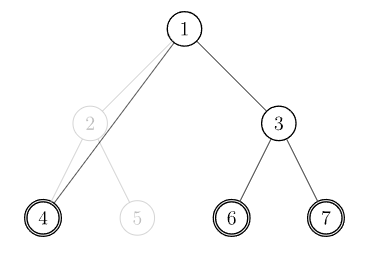
\includegraphics[width=0.5\textwidth,center]{../photo/VirtualTree}
\begin{lstlisting}[language=C++,escapeinside=``]
bool cmp(int a,int b){return dfn[a]<dfn[b];};
void dfs(int u,int fa)
{
    dfn[u]=++tim;f[u][0]=fa;dep[u]=dep[fa]+1;
    for(int i=1;i<20;i++) f[u][i]=f[f[u][i-1]][i-1];
    for(int i=head[u];~i;i=r[i].nex)
    {
        int nex=r[i].b;
        if(nex==fa) continue;
        dfs(nex,u);
    }
}
int lca(int a,int b)
{
    if(dep[a]<dep[b]) swap(a,b);
    for(int i=19;i>=0;i--)
    {
        if(dep[f[a][i]]>=dep[b])
        a=f[a][i];
    }
    if(a==b) return a;
    for(int i=19;i>=0;i--)
    {
        if(f[a][i]!=f[b][i])
        a=f[a][i],b=f[b][i]; 
    }
    return f[a][0];
}
void build_Virtual_Tree(int rt)
{
    sort(h.begin(),h.end(),cmp);
    //切记不要拿出来清空,警钟敲烂
    sta[top=1]=rt;vtree[rt].clear();
    for(int i=0;i<h.size();i++)
    {
        if(h[i]==rt) continue;
        int l=lca(sta[top],h[i]);
        //`LCA与栈顶不同,说明当前节点与栈中节点不在同一条树链上`
        if(l!=sta[top]) 
        {
            //`找到栈中与当前LCA在同一树链上的位置`
            while(dfn[sta[top-1]]>dfn[l]) 
            {
                vtree[sta[top-1]].push_back(sta[top]);
                top--;
            }
            //`这个位置不是LCA,将LCA入栈`
            if(dfn[l]>dfn[sta[top-1]]) 
            {
                vtree[l].clear();
                vtree[l].push_back(sta[top]);sta[top]=l;
            }
            else //`LCA就在栈中`
            {
                vtree[l].push_back(sta[top--]);
            }
        }
        sta[++top]=h[i];vtree[h[i]].clear();
    }
    for(int i=1;i<top;i++) 
    {
        vtree[sta[i]].push_back(sta[i+1]);
    }
}
\end{lstlisting}
\subsection{树分治}
\subsubsection{点分治}
\begin{lstlisting}[language=c++,escapeinside=``,title=求出树上两点距离小于等于$k$的点对数量]
#include<bits/stdc++.h>
using namespace std;
const int maxn=4e4+7;
int num,head[maxn],n,m,sz[maxn],w[maxn],rt,vis[maxn],dis[maxn],sum,k;
struct road{int b,c,nex;}r[80005];
void add(int a,int b,int c)
{
    r[num].b=b;r[num].c=c;r[num].nex=head[a];head[a]=num++;
}
void getrt(int u,int fa)//`找u子树中的重心`
{
    sz[u]=1;w[u]=0;
    for(int i=head[u];~i;i=r[i].nex)
    {
        int nex=r[i].b;
        if(nex==fa||vis[nex]) continue;
        getrt(nex,u);
        sz[u]+=sz[nex];
        w[u]=max(w[u],sz[nex]);
    }
    w[u]=max(w[u],sum-sz[u]);
    if(w[u]<w[rt]) rt=u;
}
int ans,cnt,a[maxn],b[maxn];
void dfs(int u,int fa,int dis,int from)
{
    b[u]=dis;a[++cnt]=b[u];
    for(int i=head[u];~i;i=r[i].nex)
    {
        int nex=r[i].b;
        if(nex==fa||vis[nex]) continue;
        dfs(nex,u,dis+r[i].c,from);
    }
}
int caldis(int u,int dis)
{
    cnt=0;b[u]=dis;a[++cnt]=b[u];
    for(int i=head[u];~i;i=r[i].nex)
    {
        int nex=r[i].b;
        if(vis[nex]) continue;
        dfs(nex,u,r[i].c+dis,nex);
    }
    int res=0;
    sort(a+1,a+1+cnt);
    for(int i=1,j=cnt;i<j;i++)
    {
        while((j-1)>i&&a[j]+a[i]>k) j--;
        if(j>i&&a[j]+a[i]<=k) res+=(j-i);
    }
    return res;
}
void solve(int u)
{
    vis[u]=1;ans+=caldis(u,0);
    for(int i=head[u];~i;i=r[i].nex)
    {
        int nex=r[i].b;
        if(vis[nex]) continue;
        ans-=caldis(nex,r[i].c);
        dis[nex]=r[i].c;
        rt=0;sum=sz[nex];
        getrt(nex,u);solve(rt);
    }
}
int main()
{
    memset(head,-1,sizeof(head));
    scanf("%d",&n);
    for(int i=1;i<n;i++)
    {
        int a,b,c;scanf("%d%d%d",&a,&b,&c);
        add(a,b,c);add(b,a,c);
    }
    scanf("%d",&k);
    w[rt]=1e9;sum=n;getrt(1,0);solve(rt);
    printf("%d\n",ans);
}
\end{lstlisting}
\section{生成树}

\subsection{次小生成树}
\noindent最小生成树转变为次小生成树,只需要插入一条新边,删去一条原边即可。\\
\noindent枚举可以插入的新边,在新边LCA的路径上找到可以删去的最长的边,可以用倍增实现。
\begin{lstlisting}[language=C++]
#include<bits/stdc++.h>
#define int long long
#define pb push_back
using namespace std;
const int maxn=3e5+7;
struct road{int x,y,c;}r[maxn];
bool cmp(road a,road b){return a.c<b.c;}
int n,m,vis[maxn],fa[maxn];
int find(int x){return fa[x]==x?x:fa[x]=find(fa[x])}
vector<pair<int,int>>v[maxn];
int f[maxn][20],mx1[maxn][20],mx2[maxn][20],depth[maxn];
void dfs(int u,int fa)
{
    depth[u]=depth[fa]+1;
    f[u][0]=fa;
    for(int i=0;i<v[u].size();i++)
    {
        auto nex=v[u][i];
        if(nex.first==fa) continue;
        mx1[nex.first][0]=nex.second;
        mx2[nex.first][0]=-1e18;
        dfs(nex.first,u);
    }
}
void ST()
{
    for(int i=1;i<20;i++)
    {
        for(int j=1;j<=n;j++)
        {
            f[j][i]=f[f[j][i-1]][i-1];
            mx1[j][i]=max(mx1[j][i-1],mx1[f[j][i-1]][i-1]);
            mx2[j][i]=max(mx2[j][i-1],mx2[f[j][i-1]][i-1]);
            if(mx1[j][i-1]!=mx1[f[j][i-1]][i-1]) 
            mx2[j][i]=max(mx2[j][i],min(mx1[j][i-1],mx1[f[j][i-1]][i-1]));
        }
    }
}
int LCA(int a,int b)
{
    if(depth[a]<depth[b]) swap(a,b);
    for(int i=19;i>=0;i--)
    {
        if(depth[f[a][i]]>=depth[b]) a=f[a][i];
    }
    if(a==b) return a;
    for(int i=19;i>=0;i--)
    {
        if(f[a][i]!=f[b][i]) a=f[a][i],b=f[b][i]; 
    }
    return f[a][0];
}
int findmx(int x,int pa,int val)
{
    int len=-1e18;
    for(int i=19;i>=0;i--)
    {
        if(depth[f[x][i]]<depth[pa]) continue;
        if(mx1[x][i]!=val) len=max(len,mx1[x][i]);
        else len=max(len,mx2[x][i]);
        x=f[x][i];
    }
    return len;
}
signed main()
{
    scanf("%lld%lld",&n,&m);
    for(int i=1;i<=n;i++) fa[i]=i;
    for(int i=1;i<=m;i++)
    {
        scanf("%lld%lld%lld",&r[i].x,&r[i].y,&r[i].c);
    }
    sort(r+1,r+1+m,cmp);
    int sum=0;
    for(int i=1;i<=m;i++)
    {
        int px=find(r[i].x),py=find(r[i].y);
        if(px==py) continue;
        vis[i]=1;fa[px]=py;sum+=r[i].c;
        v[r[i].x].pb({r[i].y,r[i].c});v[r[i].y].pb({r[i].x,r[i].c});
    }
    dfs(1,0);
    ST();
    int ans=1e18;
    for(int i=1;i<=m;i++)
    {
        if(vis[i]) continue;
        int lca=LCA(r[i].x,r[i].y);
        int lmx=findmx(r[i].x,lca,r[i].c),rmx=findmx(r[i].y,lca,r[i].c); 
        ans=min(ans,sum-max(lmx,rmx)+r[i].c);
    }
    printf("%lld\n",ans);
}
\end{lstlisting}
\subsection{瓶颈生成树}
\noindent定义:\\
\indent无向图G的瓶颈生成树是这样的一个生成树,它的最大的边权值在$G$的所有生成树中最小。\\
\noindent性质:\\
\indent\textbf{最小生成树是瓶颈生成树的充分不必要条件。}即最小生成树一定是瓶颈生成树,而瓶颈生成树不一定是最小生成树。
\subsubsection{最小瓶颈路}
\indent无向图$G$中$x$到$y$的最小瓶颈路是这样的一类简单路径,满足这条路径上的最大的边权在所有$x$到$y$的简单路径中是最小的。\\
\noindent性质:\\
\indent $x$到$y$的最小瓶颈路上的最大边权等于最小生成树上$x$到$y$路径上的最大边权。
\subsection{Kruskal重构树}
\noindent构造方法:\\
\indent在跑Kruskal的过程中我们会从小到大加入若干条边,现在我们仍然按照这个顺序。
每一次加边会合并两个集合,我们可以新建一个点,点权为加入边的边权,同时将两个集合的根节点分别设为新建点的左儿子和右儿子。
然后我们将两个集合和新建点合并成一个集合,将新建点设为根。\\
\indent不难发现,在进行$n-1$轮之后我们得到了一棵恰有$2n-1$个节点的二叉树,同时每个非叶子节点恰好有两个儿子。这棵树就叫Kruskal重构树。\\
\noindent性质:\\
\indent两点的LCA的点权为原图中最大值最小的路径上的最大值(最小瓶颈路)。\\
\indent是一颗二叉树,任意点的权值大于左右儿子的权值,是一个大根堆。\\
\\
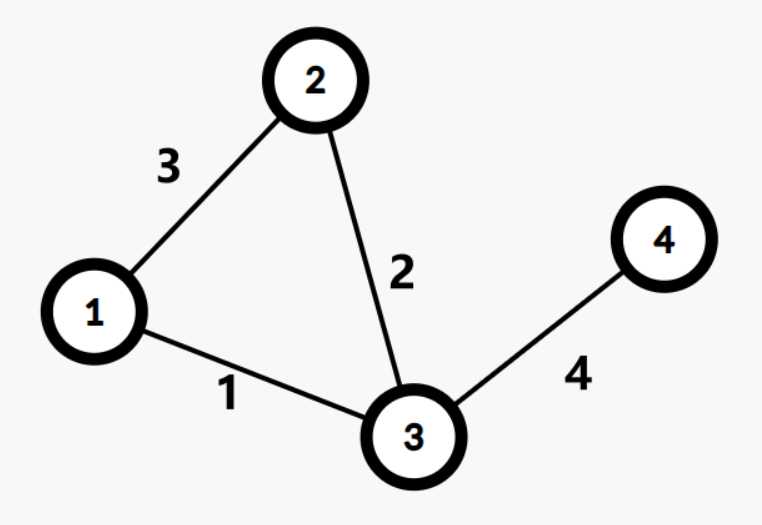
\includegraphics[width=0.5\textwidth]{../photo/kru1}
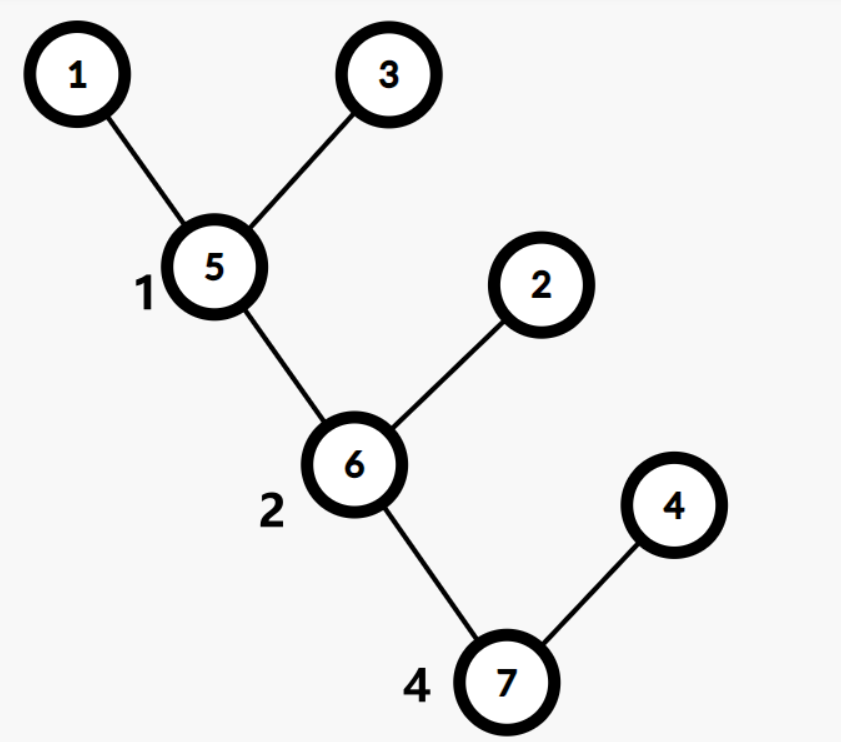
\includegraphics[width=0.5\textwidth]{../photo/kru2}
\begin{center}
    左为原图,右为该图的Kruskal重构树
\end{center}
\begin{lstlisting}[language=C++]
void Kruskal()
{
    sort(r+1,r+1+m,cmp);
    for(int i=1;i<=m;i++)
    {
        int px=find(r[i].x),py=find(r[i].y);
        if(px==py) continue;
        fa[px]=fa[py]=++idx;fa[idx]=idx;
        val[idx]=r[i].c;
        add(idx,px);add(idx,py);
    }
}
\end{lstlisting}
\section{最小树形图}
\noindent有向图上的最小生成树称为最小树形图。
\subsection{朱刘算法}
\noindent\textbf{求DAG上最小树形图:}\\
\indent对于一个$DAG$,只要我们对于每一个点选出最小的入边,那么这一定是个树形图。\\
\noindent\textbf{求环上最小树形图:}\\
\indent只需要将环上最长的一条边去掉即可。\\
\noindent\textbf{求有向图最小树形图:}\\
\indent对图上所有点直接选取其最小的入边,判断这些边是组成环。\\
\indent若无环,说明已经找到了最小树形图,直接结束即可。\\
\indent若有环,肯定要把其中一条边换成环外边。我们就把贪心算出来的那个所谓的“树形图”上的环\textbf{缩成一个点},环外边指向这个所称的点,为了方便统计,由于我们确信环外边的长度$\ge$环内边的长度,那么我们ans先加上这个环的边权和,然后指向环的边边权设为:\textbf{自己的长度$-$所连向的环内点在环中指向的点的边的长度}。\\
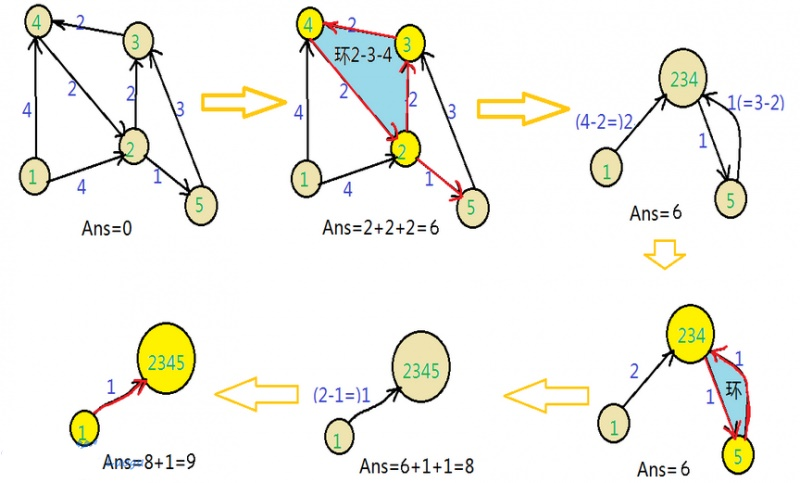
\includegraphics[width=0.8\textwidth,center]{../photo/zl.jpg}\\
\indent这样我们一直加边,找环,缩点循环,直到找到的是一个$DAG$。至此结束,时间复杂度$O(nm)$。
\begin{lstlisting}[language=c++,escapeinside=``]
int Edmonds(int root)
{
    int ans=0,cnt=0;
    while(1)
    {	//`i点的父亲是fa[i],祖先是top[i],属于第loop[i]个环,其选择的入边权值为mn[i]`
        for(int i=1;i<=n;i++) fa[i]=top[i]=loop[i]=0,mn[i]=1e9;
        for(int i=1;i<=m;i++) //找每个点最小的入边
        {
            int u=e[i].u,v=e[i].v,w=e[i].w;
            if(u!=v&&w<mn[v]) mn[v]=w,fa[v]=u;
        }
        mn[root]=0;
        for(int i=1;i<=n;i++) 
        {
            if(mn[i]==1e9) return -1; //有点无边连接,无解
            ans+=mn[i];
        }
        for(int i=1,j=1;i<=n;i++,j=i)
        {
            while(j!=root&&top[j]!=i&&!loop[j]) top[j]=i,j=fa[j];
            if(j!=root&&!loop[j]) //找到环,标号
            {
                loop[j]=++cnt;
                for(int k=fa[j];k!=j;k=fa[k]) loop[k]=cnt;
            }
        }
        if(!cnt) return ans; //如果无环,结束
        for(int i=1;i<=n;i++) if(!loop[i]) loop[i]=++cnt;//将不在环内的点设置为独立环
        for(int i=1;i<=m;i++) //缩点并且重新设置新边权
            e[i].w-=mn[e[i].v],e[i].u=loop[e[i].u],e[i].v=loop[e[i].v];
        n=cnt;root=loop[root];cnt=0; //`初始化。注意会更改n的值!!!!`
    }
}
\end{lstlisting}
\section{斯坦纳树}
\subsubsection{最小斯坦纳树}
给定连通图$G$中的$n$个点与$k$个关键点,连接$k$个关键点,使得生成树的所有边的权值和最小。\\
我们使用状态压缩动态规划来求解。用$f(i,S)$表示以$i$为根的一棵树,包含集合$S$中所有点的最小边权值和。
\begin{enumerate}
    \item 对于$i$的度数为$1$的情况,可以考虑枚举树上与$i$相邻的点$j$,则:$f(i,S)=f(j,S)+w(j,i)$。
    \item 对于$i$的度数大于$1$的情况,可以划分成几个子树考虑,即:$f(i,S)=f(i,T)+f(i,S-T)$。
\end{enumerate}
时间复杂度为$O(n\times 3^k+m\log m\times 2^k)$。
\begin{lstlisting}[language=c++]
#include<bits/stdc++.h>
using namespace std;
const int maxn=105;
typedef pair<int,int> PII;
int head[maxn],num,f[maxn][(1<<10)+5],key[10],vis[maxn];
struct road{int b,c,nex;}r[10005];
void add(int a,int b,int c)
{r[num].b=b;r[num].c=c;r[num].nex=head[a];head[a]=num++;}
priority_queue<PII,vector<PII>,greater<PII>>q;
void dijkstra(int s)
{
    memset(vis,0,sizeof(vis));
    while(!q.empty())
    {
        auto [val,u]=q.top();q.pop();
        if(vis[u]) continue;
        vis[u]=1;
        for(int i=head[u];~i;i=r[i].nex)
        {
            int v=r[i].b;
            if(f[v][s]>f[u][s]+r[i].c)
            {
                f[v][s]=f[u][s]+r[i].c;
                q.push({f[v][s],v});
            }
        }
    }
}
int main()
{
    memset(f,0x3f,sizeof(f));
    memset(head,-1,sizeof(head));
    int n,m,k;scanf("%d%d%d",&n,&m,&k);
    for(int i=1;i<=m;i++)
    {
        int a,b,c;scanf("%d%d%d",&a,&b,&c);
        add(a,b,c);add(b,a,c);
    }
    for(int i=1;i<=k;i++)
    {
        scanf("%d",&key[i]);f[key[i]][1<<(i-1)]=0;
    }
    for(int i=1;i<(1<<k);i++)
    {
        for(int j=1;j<=n;j++)
        {
            for(int sub=i&(i-1);sub;sub=i&(sub-1))
            {
                f[j][i]=min(f[j][i],f[j][sub]+f[j][i^sub]);
            }
            if(f[j][i]!=0x3f3f3f3f) q.push({f[j][i],j});
        }
        dijkstra(i);
    }
    printf("%d\n",f[key[1]][(1<<k)-1]);
}
\end{lstlisting}
\section{基环树}
\indent如果一张无向连通图包含恰好一个环,则称它是一棵基环树。\\
\indent如果一张有向弱连通图每个点的入度都为$1$,则称它是一棵基环外向树。\\
\indent如果一张有向弱连通图每个点的出度都为$1$,则称它是一棵基环内向树。
\begin{enumerate}
    \item 先处理环上每个点支出来的子树部分,然后把贡献记录在环上的点,最后问题就成了计算一个环的答案了。
    \item 先删去环上的一条边,让基环树变成真正的树计算后考虑加上之前删去那条边的影响即可(使用并查集找到环上的两个点,以两个点为树根分别树形DP)。
\end{enumerate}
\subsubsection{基环树直径}
\indent基环树的直径显然有下面两种可能:1.在“根节点”的某一棵子树中。2.经过“根节点”,在“根节点”的某两棵子树中。\\
\indent先将基环树中的环剔出来,对于环上的每棵树,使用动态规划法求出树的直径,即可解决1的可能。对于2,我们需要找到环上的两个节点$i,j$,使得$d_i+d_j+dist_{i,j}$最大。这需要我们将长度为$n$的环拓展为长度为$2*n$的链,使用单调队列维护最大的$d_j+dist_{i,j}$即可。
\begin{lstlisting}[language=c++,title=IOI2008-Island,escapeinside=``]
#include<bits/stdc++.h>
#define int long long
using namespace std;
const int maxn=1e6+7;
int head[maxn],num,n,vis[maxn],loop[2*maxn],cnt,lable[maxn],s[2*maxn];
struct road{int b,c,nex;}r[2000005];
void add(int a,int b,int c)
{
    r[num].b=b;r[num].c=c;r[num].nex=head[a];head[a]=num++;
}
bool dfs(int u,int f)
{
    if(vis[u]==1)
    {
        vis[u]=2,loop[++cnt]=u,lable[u]=1;
        return 1;
    }//找到衔接点
    vis[u]=1; //维护访问数组
    for(int i=head[u];~i;i=r[i].nex)
    {
        if(i!=(f^1)&&dfs(r[i].b,i))//如果当前边不是上一条边并且当前节点在环上
        {
            if(vis[u]!=2)//当前节点不是衔接点
            {
                loop[++cnt]=u,lable[u]=1,s[cnt]=r[i].c;
                return 1;
            } 
            else//是衔接点
            {
                s[1]=r[i].c;
                return 0;
            }
        }
    }
    return 0;	
}
int d1[maxn],d2[maxn],d;
void dfs2(int u,int fa)
{
    d1[u]=d2[u]=0;vis[u]=1;
    for(int i=head[u];~i;i=r[i].nex) 
    {
        int nex=r[i].b;
        if(nex==fa||lable[nex]) continue;
        dfs2(nex,u);
        int t=d1[nex]+r[i].c;
        if(t>d1[u]) d2[u]=d1[u],d1[u]=t;
        else if(t>d2[u]) d2[u]=t;
    }
    d=max(d,d1[u]+d2[u]);
}
signed main()
{
    memset(head,-1,sizeof(head));
    scanf("%lld",&n);
    for(int i=1;i<=n;i++)
    {
        int a,b;scanf("%lld%lld",&a,&b);
        assert(a!=i);
        add(i,a,b);add(a,i,b);
    }
    int ans=0;
    for(int i=1;i<=n;i++)
    {
        if(vis[i]) continue;
        cnt=0;dfs(i,-1);
        int sum=0;
        for(int j=1;j<=cnt;j++)
        {
            d=0;dfs2(loop[j],-1);
            sum=max(sum,d);
            s[j+cnt]=s[j];loop[j+cnt]=loop[j];
        }
        s[1]=0;
        for(int j=2;j<=2*cnt;j++) s[j]=s[j-1]+s[j];
        deque<int>q;
        for(int j=1;j<=2*cnt;j++)
        {
            while(!q.empty()&&q.front()<=j-cnt+1) q.pop_front();
            while(!q.empty()&&s[q.back()]+d1[loop[q.back()]]<=s[j]+d1[loop[j]]) 
            q.pop_back();
            q.push_back(j);
            if(j>=cnt) 
            {
                int u=q.front();
                sum=max(sum,s[u]-s[j-cnt+1]+d1[loop[u]]+d1[loop[j-cnt+1]]);
            }
        }
        ans+=sum;
    }
    printf("%lld\n",ans);
}
\end{lstlisting}
\section{搜索}
\subsection{双向搜索}
\subsubsection{双向同时搜索}
双向同时搜索的基本思路是从状态图上的起点和终点同时开始进行广搜或深搜。将起点和终点位置分别打上不同的标记,并使用搜索拓展,若某次拓展过程中遇到了不同的标记,则搜索的两端相遇了,那么可以认为是获得了可行解。
\subsubsection{meet in the middle}
主要思想是将整个搜索过程分成两半,分别搜索,最后将两半的结果合并。\\
\indent暴力搜索的时间复杂度往往是指数级别的,而改用meet in the middle算法后复杂度的指数可以减半,即让复杂度从$O(a^b)$降低成$O(a^{b/2})$。\\
\indent使用DFS同时维护模式,状态,步数基本可以较为简单的实现。
\subsection{0-1BFS}
本质是dijkstra算法,图上的边权有$0,1$两种。使用双端队列进行BFS,队首一定是队列中距离起点距离最短的点,走距离为$0/1$的边时分别将新的位置加入队首/队尾,以此来实现最短路中的松弛操作。
\subsection{A*}
A*算法是一种以BFS为基础的优化算法,在起点到终点的广阔搜索范围中,我们可以通过定义合理的启发式函数,缩小搜索的范围,从而加速搜索。\\
\indent定义起点为$s$,终点为$t$,从起点(初始状态)开始的真实距离为$d(x)$,到终点(最终状态)的真实距离$h(x)$,估计距离为$h^{*}(x)$,必须满足$h^{*}(x)\leq h(x)$,以及每个点的估价函数$f(x)=d(x)+h^{*}(x)$。\\
\indent A*算法每次从优先队列中取出一个$f$最小的元素,然后更新相邻的状态。在启发式函数的约束下,搜索效率得以提升,当\textbf{终点第一次离开队列时},此时记录的便是最优答案。\\
\indent当$h=0$时,A*算法变为 Dijkstra,当$h=0$并且边权为$1$时变为BFS。
\subsubsection{八数码问题}
\indent题目大意:在$3\times3$的棋盘上,摆有八个棋子,每个棋子上标有$1$至$8$的某一数字。棋盘中留有一个空格,空格用$0$来表示。空格周围的棋子可以移到空格中,这样原来的位置就会变成空格。给出一种初始布局和目标布局(为了使题目简单,设目标状态如下),找到一种从初始布局到目标布局最少步骤的移动方法。\\
\indent启发式函数$h$定义为,不在应该在的位置的数字个数。
\begin{lstlisting}[language=C++]
#include<bits/stdc++.h>
using namespace std;
string ed="123804765",st;
int h(string s)
{
    int cnt=0;
    for(int i=0;i<9;i++) cnt+=(s[i]!=ed[i]);
    return cnt;
}
map<string,int>vis;
int nex[4]={-3,3,-1,1};
struct node
{
    string str;int v;
    bool operator<(node x)const{return x.v+h(x.str)<v+h(str);}
};
int main()
{
    cin>>st;
    priority_queue<node>q;
    q.push({st,0});
    int ans;
    while(!q.empty())
    {
        string sta=q.top().str;
        int step=q.top().v;q.pop();
        if(sta==ed)
        {
            ans=step;break;
        }
        int pos;
        for(int i=0;i<9;i++) if(sta[i]=='0') pos=i;
        for(int i=0;i<4;i++)
        {
            if((i==0&&pos/3==0)||(i==1&&pos/3==2)||(i==2&&pos%3==0)||(i==3&&pos%3==2))
            continue;
            string temp=sta;swap(temp[pos],temp[pos+nex[i]]);
            if(!vis.count(temp))
            {
                vis[temp]=1;q.push({temp,step+1});
            }
        }
    }
    printf("%d\n",ans);
}
\end{lstlisting}
\subsubsection{K短路}
启发式函数为$f(x)=d(x)+dis(x)$,$dis(x)$为$x$点到终点的最短路距离,当终点第一次出队时为最短路,第$k$次出队时的距离即为第$k$短路。使用A*算法时间复杂度为$O(nk\log n)$,存在使用可持久化可并堆的算法可以做到在$O((n+m) \log n + k \log k)$的时间复杂度解决$k$短路问题。
\begin{lstlisting}[language=C++]
#include<bits/stdc++.h>
using namespace std;
typedef pair<double,int> PDI;
const int maxn=5005;
int n,m,num,h[maxn],h1[maxn],vis[maxn];
double sum,dis[maxn];
struct road{int b,nex;double c;}r[400005];
void add(int a,int b,double c){r[num].b=b;r[num].c=c;r[num].nex=h[a];h[a]=num++;}
void add1(int a,int b,double c){r[num].b=b;r[num].c=c;r[num].nex=h1[a];h1[a]=num++;}
void dijkstra(int num)
{
    for(int i=1;i<=n;i++) dis[i]=1e9;
    priority_queue<PDI,vector<PDI>,greater<PDI>>q;
    dis[num]=0;q.push({0,num});
    while(!q.empty())
    {
        int d=q.top().second;double v=q.top().first;q.pop();
        if(vis[d]) continue;vis[d]=1;
        for(int i=h1[d];~i;i=r[i].nex)
        {
            int nex=r[i].b;double val=r[i].c;
            if(dis[nex]>dis[d]+val)
            {
                dis[nex]=dis[d]+val;
                q.push({dis[nex],nex});
            }
        }
    }
}
struct node
{
    int p;double s;
    bool operator<(node x)const{return x.s+dis[x.p]<s+dis[p];}
};
int astar()
{
    priority_queue<node>q;q.push({1,0});
    int ans=0;
    while(!q.empty())
    {
        int pos=q.top().p;double step=q.top().s;q.pop();
        if(pos==n)
        {
            if(sum>=step) sum-=step,ans++;
            else break;
        }
        for(int i=h[pos];~i;i=r[i].nex)
        {
            int nex=r[i].b;q.push({nex,r[i].c+step});
        }
    }
    return ans;
}
int main()
{
    memset(h,-1,sizeof(h));
    memset(h1,-1,sizeof(h1));
    scanf("%d%d%lf",&n,&m,&sum);
    for(int i=1;i<=m;i++)
    {
        int a,b;double w;
        scanf("%d%d%lf",&a,&b,&w);
        add(a,b,w);add1(b,a,w);
    }
    dijkstra(n);
    printf("%d\n",astar());
}
\end{lstlisting}
\subsection{迭代加深}
\indent迭代加深是一种\textbf{每次限制搜索深度的}深度优先搜索。迭代加深在搜索的同时带上了一个深度$d$,当$d$达到设定的深度时就返回,一般用于找最优解。如果一次搜索没有找到合法的解,就让设定的深度加一,重新从根开始。\\
\indent可以认为迭代加深是一种使用DFS实现BFS的过程,相较于BFS队列记录信息较多时会占用较大的内存,迭代加深空间复杂度相对较小。
\begin{lstlisting}[language=c++,title=UVA529 Addition Chains]
#include<bits/stdc++.h>
using namespace std;
int n,ans[100],lim;
bool dfs(int u)
{
    if(u>lim) return ans[u-1]==n;
    if(ans[u-1]*(1<<(lim-u+1))<n) return false;
    for(int i=1;i<u;i++)
    {
        for(int j=i;j<u;j++)
        {
            if(ans[i]+ans[j]>n) break;
            ans[u]=ans[i]+ans[j];
            if(dfs(u+1)) return true;
        }
    }
    return false;
}
int main()
{
    while(scanf("%d",&n)!=EOF&&n)
    {
        ans[1]=1;lim=1;
        while(!dfs(2)) lim++;
        for(int i=1;i<=lim;i++) printf("%d ",ans[i]); 
        puts("");
    }
}
\end{lstlisting}
\subsection{IDA*}
\indent本质上是迭代加深DFS和A*的结合。整个过程较为简单,构造合适的启发式函数,在使用迭代加深搜素时,用启发式函数判断距离,从而快速减枝。
\section{拓扑排序}
\begin{lstlisting}[language=C++,title=拓扑排序找环]
bool topsort()
{
    int cnt=0;queue<int>q;
    for(int i=1;i<=n;i++) if(d[i]==0) q.push(i),cnt++;			
    while(!q.empty())
    {
        int k=q.front();q.pop();
        for(int i=head[k];~i;i=r[i].nex)
        {
            int v=r[i].b;
            if(--d[v]==0)
            {
                q.push(v);cnt++;
            } 
        }
    } 
    return cnt==n;
}
\end{lstlisting}

\section{最短路}
\subsection{Dijkstra}
\begin{lstlisting}[language=C++]
void dijkstra(int num)
{
    priority_queue<PII,vector<PII>,greater<PII> >q;
    dis[num]=0;
    q.push({0,num});
    while(!q.empty())
    {
        PII p=q.top(); q.pop();
        int d=p.second,v=p.first;
        if(vis[d]) continue;
        vis[d]=1;
        for(int i=head[d];~i;i=r[i].nex)
        {
            int next=r[i].b,val=r[i].c;
            if(dis[next]>dis[d]+val)
            {
                dis[next]=dis[d]+val;
                q.push({dis[next],next});
            }
        }
    }
}
\end{lstlisting}

\subsection{SPFA}
\begin{lstlisting}[language=C++]
bool spfa(int num)
{
    queue<int>q;dis[num]=0;
    q.push(num);vis[num]=1;
    while(!q.empty())
    {
        int k=q.front();q.pop();vis[k]=0;
        for(int i=head[k];~i;i=r[i].nex)
        {
            if(dis[r[i].b]>dis[k]+r[i].c)
            {
                dis[r[i].b]=dis[k]+r[i].c;
                cnt[r[i].b]=cnt[k]+1;
                if(cnt[r[i].b]>n) return false;
                if(vis[r[i].b]==0)
                {
                    q.push(r[i].b);
                    vis[r[i].b]=1;
                }	
            }
        }
    }
    return true;
}
\end{lstlisting}
\subsubsection{SPFA其余形式优化}
普通SPFA是非常好卡的,只需要一个随机网格图(在网格图中走错一次路可能导致很高的额外开销),或者一个构造过的链套菊花(使得队列更新菊花的次数非常高)即可。很多奇怪写法的SPFA都只能通过两者中的至多一种,因此你只需要将图构造为网格套菊花即可。\\
\indent\textbf{堆优化}:将队列换成堆,与Dijkstra的区别是允许一个点多次入队。在有负权边的图可能被卡成指数级复杂度。\\
\indent\textbf{栈优化}:将队列换成栈(即将原来的BFS过程变成 DFS),在寻找负环时可能具有更高效率,但最坏时间复杂度仍然为指数级。\\
\indent\textbf{LLL优化}:将普通队列换成双端队列,每次将入队结点距离和队内距离平均值比较,如果更大则插入至队尾,否则插入队首。\\
\indent\textbf{SLF优化}:将普通队列换成双端队列,每次将入队结点距离和队首比较,如果更大则插入至队尾,否则插入队首。\\
\indent\textbf{D´Esopo-Pape 算法}:将普通队列换成双端队列,如果一个节点之前没有入队,则将其插入队尾,否则插入队首。

\subsection{差分约束}
\noindent\textbf{求最大值:}\\
\indent按照$B-A\leq W$进行不等式的转化add(a,b,w),求出图中的最短路,即为最大值。\\
\noindent\textbf{求最小值:}\\
\indent按照$B-A\ge w$进行不等式的转化add(a,b,w),最长路即为最小值。\\
\noindent如果图中存在负环/正环,则不等式无法成立。\\
\indent差分约束找环求最值不一定非要使用SPFA求最短路求解,对于边权均为正/负的图,可以先用Tarjan判环缩点为DAG后使用拓扑排序求解。

\subsection{同余最短路}
\indent当出现形如“给定$n$个整数,求这$n$个整数能拼凑出多少的其他整数($n$个整数可以重复取)”,以及“给定$n$个整数,求这$n$个整数不能拼凑出的最小(最大)的整数”,或者“至少要拼几次才能拼出模$K$余$p$的数”的问题时可以使用同余最短路的方法。\\
\indent对于$x,y,z$三个数字能够拼凑出来的小于$h$的数字,令$dis_i$为只使用$y$和$z$,能得到的模$x$下与$i$同余的最小数,用来计算该同余类满足条件的数个数。\\
\indent于是可以有以下转移:$\begin{cases}i\xrightarrow{y}(i+y)\bmod x \\ i\xrightarrow{z}(i+z)\bmod x\end{cases}$\\
\indent相当于在在图上建边$\begin{cases}add(i,(i+y) \% x, y)\\add(i, (i+z) \% x, z)\end{cases}$\\
\indent接下来只需要对整个图跑最短路,得到所有的$dis$,最后的答案即为:\\
$$
\sum_{i=0}^{x-1}\left(\frac{h-d_i}{x}+1\right)
$$
\begin{lstlisting}[language=C++]
#include<bits/stdc++.h>
using namespace std;
typedef pair<long long,int> PII;
const int maxn=1e5+7;
int x,y,z,num,head[maxn],vis[maxn];
long long h,dis[maxn];
struct road{int b,c,nex;}r[2000005];
void add(int a,int b,int c)
{r[num].b=b;r[num].c=c;r[num].nex=head[a];head[a]=num++;}
void dijkstra(int num)
{
    memset(dis,0x3f3f,sizeof(dis));
    priority_queue<PII,vector<PII>,greater<PII> >q;
    dis[num]=0;q.push({0,num});
    while(!q.empty())
    {
        PII p=q.top(); q.pop();
        int d=p.second,v=p.first;
        if(vis[d]) continue;
        vis[d]=1;
        for(int i=head[d];~i;i=r[i].nex)
        {
            int next=r[i].b,val=r[i].c;
            if(dis[next]>dis[d]+val)
            {
                dis[next]=dis[d]+val;
                q.push({dis[next],next});
            }
        }
    }
}
int main()
{
    memset(head,-1,sizeof(head));
    scanf("%lld%d%d%d",&h,&x,&y,&z);
    if(x==1)//注意特判
    {
        printf("%lld\n",h);
        return 0;
    }
    for(int i=0;i<x;i++)
    {
        add(i,(i+y)%x,y);add(i,(i+z)%x,z);
    }
    dijkstra(0);
    long long ans=0;
    for(int i=0;i<x;i++) 
    {
        if(h>=dis[i]) ans+=((h-dis[i])/x+1);
    }
    printf("%lld\n",ans);
}
\end{lstlisting}
\section{欧拉图}
\noindent\textbf{定义:}\\
\indent通过图中所有边恰好一次的通路称为欧拉通路。\\
\indent通过图中所有边恰好一次的回路称为欧拉回路。\\
\indent具有欧拉回路的无向图或有向图称为欧拉图。\\
\indent具有欧拉通路但不具有欧拉回路的无向图或有向图称为半欧拉图。\\
\indent非形式化地讲,欧拉图就是从任意一个点开始都可以一笔画完整个图,半欧拉图必须从某个点开始才能一笔画完整个图。\\
\noindent\textbf{性质:}\\
\indent欧拉图中所有顶点的度数都是偶数。\\
\indent若$G$是欧拉图,则它为若干个环的并,且每条边被包含在奇数个环内。\\
\noindent\textbf{辨别法:}\\
\noindent对于无向图(图是连通图):\\
\indent欧拉通路的充要条件:度数为奇数的点只能有$0$个或$2$个。\\
\indent欧拉回路的充要条件:度数为奇数的点只能有$0$个。\\
\noindent对于有向图(图是连通图):\\
\indent欧拉通路的充要条件:要么所有点的入度等于出度,要么除了两个点外所有点的入度等于出度,这两个点一个出度比入度多$1$(起点),一个入度比出度多$1$(终点)。\\
\indent欧拉回路的充要条件:所有点的入度等于出度。
\subsection{Fleury算法}
\indent也称避桥法,是一个偏暴力的算法。\\
\indent算法流程为每次选择下一条边的时候优先选择不是桥的边。\\
\indent一个广泛使用但是错误的实现方式是先Tarjan预处理桥边,然后再DFS避免走桥。但是由于走图过程中边会被删去,一些非桥边会变为桥边导致错误。最简单的实现方法是每次删除一条边之后暴力跑一遍Tarjan找桥,时间复杂度是$O(m^2)$。复杂的实现方法要用到动态图等,实用价值不高。
\subsection{Hierholzer算法}
\begin{lstlisting}[language=c++,title=无向图欧拉回路字典序最小输出方案]
struct node
{
    int to,exit,rev;
    bool operator<(node x)const{return to<x.to;}
};
vector<node>v[maxn];
vector<int>ans;
void dfs(int u)
{
    for(int i=head[u];i<v[u].size();i=head[u])
    {
        if(v[u][i].exit)
        {
            node e=v[u][i];
            v[u][i].exit=0;v[e.to][e.rev].exit=0;
            head[u]++;
            dfs(e.to);
        }
        else head[u]++;
    }
    ans.push_back(u);
}
int revtop[maxn];
int main()
{
    scanf("%d",&m);
    for(int i=1;i<=m;i++)
    {
        int a,b;scanf("%d%d",&a,&b);
        v[a].push_back({b,1,0});v[b].push_back({a,1,0});
        d[a]++;d[b]++;
    }
    for(int i=1;i<=n;i++) sort(v[i].begin(),v[i].end());
    for(int i=1;i<=n;i++) 
    {
        for(int j=0;j<v[i].size();j++) v[i][j].rev=revtop[v[i][j].to]++;
    }
    int st=1;
    for(int i=1;i<=n;i++) if(d[i]%2){st=i;break;}
    dfs(st);
    reverse(ans.begin(),ans.end());
    for(auto i:ans) printf("%d\n",i);
}
\end{lstlisting}
\subsection{混合图欧拉回路}
\indent将所有无向边任意规定一个方向,统计各点的度数,若某点入度出度和为奇数,则不存在欧拉回路。\\
\indent满足上述条件后,删除原图中的有向边,用网络流建图。\\
\indent对出度大于入度的点,用源点向其连接大小为需要改变的边数的边。对入度大于出度的点,用汇点向其连接大小为需要改变的边数的边,其余规定了方向的无向边在网络流图上流量为$1$。跑网络流,如果可以满流,则说明存在欧拉回路,满流的边意味着该无向边需要反转方向。
\section{哈密顿图}
\noindent\textbf{定义:}\\
\indent通过图中所有顶点一次且仅一次的通路称为哈密顿通路。\\
\indent通过图中所有顶点一次且仅一次的回路称为哈密顿回路。\\
\indent具有哈密顿回路的图称为哈密顿图。具有哈密顿通路而不具有哈密顿回路的图称为半哈密顿图。

\section{连通图}
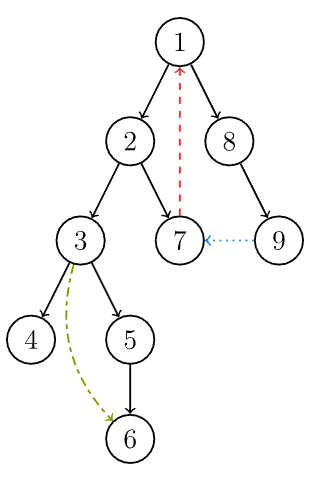
\includegraphics[width=0.3\textwidth,center]{../photo/dfstree}
\indent一颗DFS生成树包含四种类型的边,\textbf{树边,返祖边,横叉边,前向边}。\\
\indent定义DFN(u)为节点u搜索的次序编号(时间戳),Low(u)为u或u的子树能够追溯到的最早的\textbf{栈中}节点的次序号。
\subsection{强连通分量}
\begin{lstlisting}[language=C++]
void tarjan(int u)
{
    dfn[u]=low[u]=++tim;
    atack.push(u);inst[u]=1;
    for(int i=head[u];~i;i=r[i].nex)
    {
        int v=r[i].b;
        if(dfn[v]==0)
        {
            tarjan(v);low[u]=min(low[u],low[v]);
        }
        else if(inst[v]==1) low[u]=min(low[u],dfn[v]);
    }
    if(dfn[u]==low[u])
    {
        numb++;int q;
        do
        {
            q=atack.top();inst[q]=0;atack.pop();
            bl[q]=numb;nums[numb]++;
        }while(q!=u);
    }
}
\end{lstlisting}
将多个强连通分量加边联通为一个强连通分量,最少需要$\max (num_{ru=0},num_{chu=0})$条边,只有一个强连通分量需要特判。
\subsection{双连通分量}
只要删去桥还能够保持联通,就是边双连通。
\begin{lstlisting}[language=C++,title=边双连通分量]
void tarjan(int u,int f)//f是路线编号
{
    atack.push(u);
    dfn[u]=low[u]=++tim;
    for(int i=head[u];~i;i=r[i].nex)
    {
        int v=r[i].b;
        if(!dfn[v])
        {
            tarjan(v,i);low[u]=min(low[u],low[v]);
        }
        else if(i!=(f^1)) low[u]=min(low[u],dfn[v]);
    }
    if(dfn[u]==low[u])
    {
        numb++;int t;
        do
        {
            t=atack.top();atack.pop();
            bl[t]=numb;nums[numb]++;
        }while(t!=u);
    }
}
\end{lstlisting}
只要删去割点还能保持联通,就是点双连通,但是要注意,一个割点可能同时属于多个点双连通分量。\textbf{注意特判自环!!!!}
\begin{lstlisting}[language=C++,title=点双连通分量]
void tarjan(int u,int root)//有没有fa其实无所谓
{
    dfn[u]=low[u]=++tim;
    atack.push(u);
    if(u==root && head[u]==-1)//特判孤立点
    {
        dcc[++numb].push_back(u);return;
    }
    int child=0;
    for(int i=head[u];~i;i=r[i].nex)
    {
        int v=r[i].b;
        if(!dfn[v])
        {
            tarjan(v,root);
            low[u]=min(low[u],low[v]);
            if(dfn[u]==low[v])
            {
                child++;
                if(u!=root||child>1) isgd[u]=true;
                numb++;
                int y;
                do{
                    y=atack.top();atack.pop();
                    dcc[numb].push_back(y);
                }while(y!=v);
                dcc[numb].push_back(u);
            }
        }
        else low[u]=min(low[u],dfn[v]);
    }
}
\end{lstlisting}
\subsection{割点和桥}
将某点及其连边删去,图无法继续连通。
\begin{lstlisting}[language=C++,title=割点]
void tarjan(int u,int root)
{
    dfn[u]=low[u]=++tim;
    int child=0;
    for(int i=head[u];~i;i=r[i].nex)
    {
        int v=r[i].b;
        if(!dfn[v])
        {
            tarjan(v,root);
            low[u]=min(low[u],low[v]);
            if(low[v]==dfn[u])
            {
                child++;
                if(u!=root || child>1)	isgd[u]=1;
            }
        }
        else
        low[u]=min(low[u],dfn[v]);
    }
}
\end{lstlisting}
删去图中的某个边,图不再连通,无向图只包含树边和非树边,没有非树边覆盖的树边就是桥。
\begin{lstlisting}[language=C++,title=桥]
void tarjan(int u,int f)//f是路线编号
{
    dfn[u]=low[u]=++tim;
    for(int i=head[u];~i;i=r[i].nex)
    {
        int v=r[i].b;
        if(!dfn[v])
        {
            tarjan(v,i);
            low[u]=min(low[u],low[v]);
            if(dfn[u]<low[v])//和割点的区别
            {
                isbri[i]=isbri[i^1]=1;
            }
        }
        else if(i!=(f^1))
        low[u]=min(low[u],dfn[v]);
    }
}
\end{lstlisting}
一棵树上有$n$个度数为$1$的点,最少连接$(n+1)/2$条边即可变为双连通分量。
\subsection{圆方树}
\indent众所周知,树(或森林)有很好的性质,并且容易通过很多常见数据结构维护。\\
\indent而一般图则没有那么好的性质,所幸有时我们可以把一般图上的某些问题转化到树上考虑。\\
\indent顾名思义,圆方树即有圆点有方点的树。\\
\indent在一张无向图中,将图中原有的点视为圆点,将图中的点双连通分量视为一个方点,将方点对应的圆点用菊花图的连接方式连接起来。就会形成一颗(或多颗)圆方树(森林)。\\
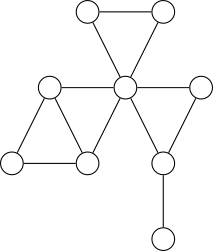
\includegraphics[width=0.33\textwidth]{../photo/yfs1.png}
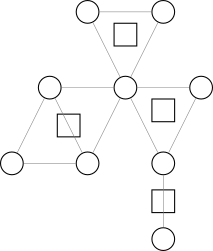
\includegraphics[width=0.33\textwidth]{../photo/yfs2.png}
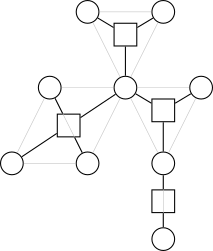
\includegraphics[width=0.33\textwidth]{../photo/yfs3.png}
\noindent\textbf{技巧:}\\
\indent1.对圆方树上圆点权值初始化为$-1$,方点权值初始化为度数大小。任意两圆点在树上路径权值之和即为原无向图两点路径途经点集的数量和。
\indent2.无向图任意两点间的割点数,等价于圆方树上两点树上路径上的圆点数量。
\begin{lstlisting}
void tarjan(int u)
{
    dfn[u]=low[u]=++tim;
    stk.push(u);
    for(int i=head[u];~i;i=r[i].nex)
    {
        int v=r[i].b;
        if(!dfn[v])
        {
            tarjan(v);low[u]=min(low[u],low[v]);
            if(low[v]==dfn[u])
            {
                idx++;int x;
                do
                {
                    x=stk.top();stk.pop();
                    rst[idx].push_back(x);
                    rst[x].push_back(idx);
                }while(x!=v);
                rst[u].push_back(idx);
                rst[idx].push_back(u);
            }
        }
        else low[u]=min(low[u],dfn[v]);
    }
}
\end{lstlisting}
\section{仙人掌}
仙人掌图(cactus)是一种无向连通图,它的每条边最多只能出现在一个简单回路里面。从直观上说,可以把仙人掌图理解为允许存在回路的树。如果一个图不包含\textbf{偶数环}那么这个图一定是仙人掌。\\
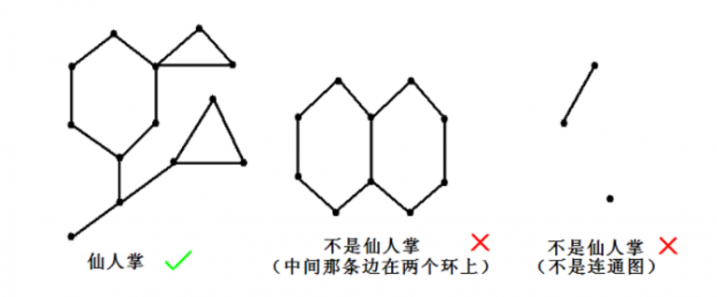
\includegraphics[width=0.5\textwidth,center]{../photo/xrz.png}
\subsubsection{仙人掌圆方树}
上述圆方树在某种意义上被认为是广义圆方树,即适用于一般无向图的圆方树。对于仙人掌,我们对其使用狭义圆方树。两种圆方树一个明显的区别就是,一个只有两个点的点双联通分量要不要建方点。因此除了广义圆方树上仅有的圆方边,在此类圆方树中还包含圆圆边,但两种圆方树中都不存在方方边。\\
\indent仙人掌图本质上是一个树上开花(环)的树,因此我们对其做边双连通分量,对于树边(桥),继续用原图上的边对其连接(圆圆边),如果遇到了环,对环上节点依次与其方点连接。建好的树即为仙人掌圆方树。\\
\subsubsection{仙人掌上最短路}
对于圆圆边,边权为原边边权,圆方边的边权为$0$,方圆边的边权为原图上圆点到方点父亲的最短路。\\
\indent建好树后,记$dis(x)$为$x$点到树根的距离,对于$u$到$v$的最短路,若其LCA为圆点,最短路即$dis(u)+dis(v)-2*dis(LCA)$。若为方点,找出LCA的两个儿子$A,B$,分别为$u,v$的祖先,此时最短路即$dis(A,B)+dis(u,A)+dis(v,B)$。其中$dis(A,B)$可以通过预处理环长计算。
\begin{lstlisting}[language=c++]
#include<bits/stdc++.h>
using namespace std;
typedef long long ll;
const int maxn=20005;
int n,m,q,f[maxn][16],head[maxn],dep[maxn],num,dfn[maxn],low[maxn],tim,idx;
int sum[maxn],len[maxn],fa[maxn],dis[maxn],A,B;
struct road{int b,c,nex;}r[2000005];
void add(int a,int b,int c){r[num].b=b;r[num].c=c;r[num].nex=head[a];head[a]=num++;}
stack<int>stk;
vector<pair<int,int>>rst[maxn];
void build_tree(int u,int v,int val)
{
    int pre=val,x=v;
    while(x!=fa[u])
    {
        sum[x]=pre;pre+=len[x];x=fa[x];
    }
    sum[++idx]=sum[u];
    x=v;rst[u].push_back({idx,0});
    while(x!=u)
    {
        int mn=min(sum[idx]-sum[x],sum[x]);
        rst[idx].push_back({x,mn});x=fa[x];
    }
}
void tarjan(int u,int from)
{
    dfn[u]=low[u]=++tim;
    stk.push(u);
    for(int i=head[u];~i;i=r[i].nex)
    {
        int v=r[i].b;
        if(!dfn[v])
        {
            len[v]=r[i].c;fa[v]=u;
            tarjan(v,i);
            low[u]=min(low[u],low[v]);
        }
        else if(i!=(from^1)) low[u]=min(low[u],dfn[v]);
        if(low[v]>dfn[u]) //桥=圆圆边
        {
            rst[u].push_back({v,r[i].c});
        }
    }
    for(int i=head[u];~i;i=r[i].nex)
    {
        int v=r[i].b;
        if(fa[v]==u||dfn[v]<=dfn[u]) continue;
        build_tree(u,v,r[i].c);
    }
}
void dfs(int u,int fa)
{
    f[u][0]=fa;dep[u]=dep[fa]+1;
    for(int i=1;i<=15;i++) f[u][i]=f[f[u][i-1]][i-1];
    for(auto [nex,w]:rst[u])
    {
        dis[nex]=dis[u]+w;
        dfs(nex,u);
    }
}
int lca(int a,int b)
{
    if(dep[a]<dep[b]) swap(a,b);
    for(int i=15;i>=0;i--)
    {
        if(dep[f[a][i]]>=dep[b]) a=f[a][i];
    }
    if(a==b) return a;
    for(int i=15;i>=0;i--)
    {
        if(f[a][i]!=f[b][i]) a=f[a][i],b=f[b][i]; 
    }
    A=a,B=b;
    return f[a][0];
}
int main()
{
    memset(head,-1,sizeof(head));
    scanf("%d%d%d",&n,&m,&q);idx=n;
    for(int i=1;i<=m;i++)
    {
        int u,v,w;scanf("%d%d%d",&u,&v,&w);
        add(u,v,w);add(v,u,w);
    }
    tarjan(1,-1);
    dfs(1,0);
    while(q--)
    {
        int a,b;scanf("%d%d",&a,&b);
        int LCA=lca(a,b);
        if(LCA<=n) printf("%d\n",dis[a]+dis[b]-2*dis[LCA]);
        else printf("%d\n",dis[a]+dis[b]-dis[A]-dis[B]+min(abs(sum[A]-sum[B]),sum[LCA]-abs(sum[A]-sum[B])));
    }
}
\end{lstlisting}


\section{2-SAT}
\indent个人认为2-SAT跟强连通的关系有点像差分约束跟最短路的关系。\\
\indent\textbf{k-SAT问题}:有$n$个$bool$类型的事件,有$m$种约束,每种约束都有$k$个事件的关系。找出一种符合约束的$n$个事件的取值。(NP完全问题)\\
\indent将$n$个事件拆分为$2*n$个点,分别代表$0,1$两种情况。对于所有的约束,我们根据题意建立有向图。若在有向图中有$(a\Rightarrow b)$,则意为选择了$a$一定要同时选择$b$才可以满足约束条件。\\
\indent根据题意建好图后,应首先判断事件约束是否合法。对其进行\textbf{强连通分量缩点},若$a,b$在同一个强连通分量内,则意味着$a,b$绑定在了一起,必须同时选取才能满足约束。这种情况下,如果某个事件的$0,1$情况在同一个强连通分量下,该事件就又要为$1$又要为$0$,显然这是矛盾的。\\
\indent在判断完上述情况后,就一定存在满足约束要求的合法方案。优先选择强连通分量标号较小的情况,因为在Tarjan结束后的出栈顺序决定了缩点后DAG的拓扑序。
\begin{center}
\begin{tabular}{|c|c|}
\hline 
原式 & 构图\\
\hline 
$a\lor b=1$ & $(\neg a\Rightarrow b)\land(\neg b\Rightarrow a)$\\
\hline 
$a \& b=1$ & $(\neg a\Rightarrow a)\land(\neg b\Rightarrow b)$ \\
\hline 
$a \& b=0$ & $(a\Rightarrow \neg b)\land(b\Rightarrow \neg a)$ \\
\hline
$a \mid b=1$ & $(\neg a\Rightarrow b)\land(\neg b\Rightarrow a)$  \\
\hline
$a \mid b=0$ & $(a\Rightarrow \neg a)\land(b\Rightarrow \neg b)$\\
\hline
$a\oplus b=1$ & $(a\Rightarrow \neg b)\land(\neg a\Rightarrow b)\land(b \Rightarrow \neg a)\land(\neg b\Rightarrow a)$\\
\hline
$\quad a\oplus b=0 \quad$ & $\quad (a\Rightarrow b)\land(\neg a\Rightarrow \neg b)\land(b \Rightarrow a)\land(\neg b\Rightarrow \neg a)\quad$\\
\hline
\end{tabular}    
\end{center}

\begin{lstlisting}[language=c++]
for(int i=1;i<=n;i++)
{
    if(bl[i]==bl[i+n]){puts("IMPOSSIBLE");return 0;}
}
puts("POSSIBLE");
for(int i=1;i<=n;i++)
{
    if(bl[i]<bl[i+n]) printf("1 ");
    else printf("0 ");
}
\end{lstlisting}

\section{图的匹配}
\begin{itemize}
    \item 最大匹配: 匹配数最多的匹配。
    \item 完美匹配: 所有点都属于匹配,同时也符合最大匹配。
    \item 近完美匹配: 发生在图的点数为奇数,刚好只有一个点不在匹配中。
\end{itemize}
\subsubsection{增广路定理}
\indent交错路:始于非匹配点且由匹配边与非匹配边交错而成。\\
\indent增广路:是始于非匹配点且终于非匹配点的交错路。\\
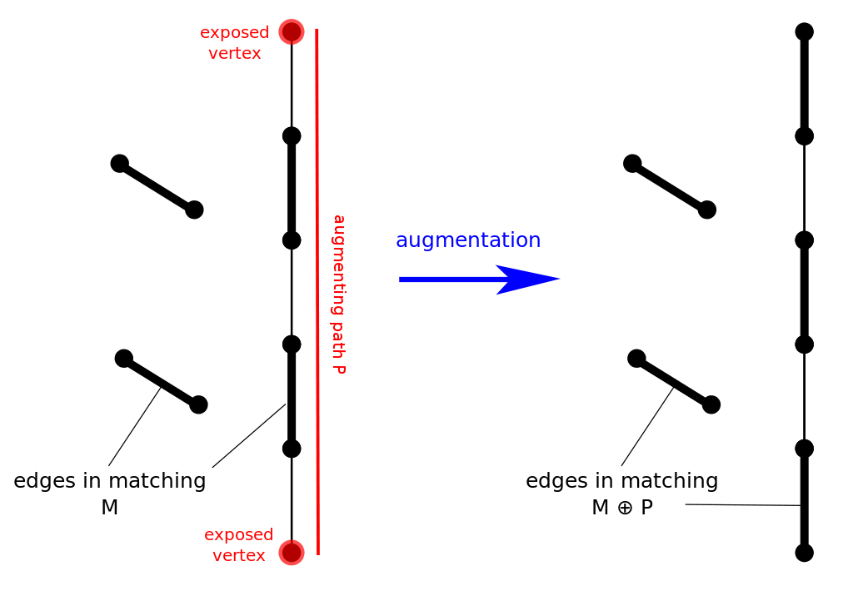
\includegraphics[width=0.5\textwidth,center]{../photo/Berge's lemma}\\
\indent增广路上非匹配边比匹配边数量多一,如果将匹配边改为未匹配边,反之亦然,则匹配大小会增加一且依然是交错路。
\subsection{二分图}
\subsubsection{染色法判断二分图}
\begin{lstlisting}[language=c++]
bool dfs(int u,int color)
{
    col[u]=color;
    for(int i=head[u];~i;i=r[i].nex)
    {
        int next=r[i].b;
        if(col[next]==0)
        {
            if(!dfs(next,3-color)) return false;
        }
        else
        {
            if(col[next]==color) return false;
        }
    }
    return true;
}
\end{lstlisting}
\subsubsection{二分图完美匹配}
设$G=<V_1,V_2,E>$为二分图,$|V_1|\leq|V_2|$,$M$为$G$中一个最大匹配,且$M=|V_1|$,则称$M$为$V_1$到$V_2$的完美匹配。
\subsubsection{霍尔定理}
对于一个二分图,如果对于左边任意子集$S$,其对应边连接了一个右边的边集$T$,都有$|S|<=|T|$,那么这个二分图有完美匹配(充要)。
\subsection{二分图最大匹配}
\subsubsection{匈牙利算法}
\begin{lstlisting}[language=c++,title=邻接矩阵$O(n^3)$]
bool match(int x)
{
    for(int i=1;i<=n2;i++)
    {
        if(side[x][i]&&!vis[i])
        {
            vis[i]=1; //将i加入增广路上
            if(!mat[i]||match(mat[i])) 
            {
                mat[i]=x;return true;
            }
        }
    }
    return false;
}
int Hungarian()
{
    int ans=0;
    for(int i=1;i<=n1;i++)
    {
        memset(vis,0,sizeof(vis));
        if(match(i)) ans++;
    }
    return ans;
}
\end{lstlisting}
\begin{itemize}
    \item 换用邻接表,可将时间优化至$O(nm)$,使用网络流建图跑dinic,时间复杂度$O(m\sqrt n)$。
    \item 若同侧匹配,记得反向记录mat,且第一次开始递归的节点$x$标记vis[x]=1。
\end{itemize}
\subsubsection{二分图最小点覆盖(König 定理)}
\indent最小点覆盖:选最少的点,满足每条边至少有一个端点被选。\\
\indent二分图中,最小点覆盖$=$最大匹配。
\subsubsection{二分图最大独立集}
\indent最大独立集:选最多的点,满足两两之间没有边相连。\\
\indent因为在最小点覆盖中,任意一条边都被至少选了一个顶点,所以对于其点集的补集,任意一条边都被至多选了一个顶点,所以不存在边连接两个点集中的点,且该点集最大。因此二分图中,最大独立集$=$总点$-$最小点覆盖。
\subsection{二分图最大权匹配}
\subsubsection{KM算法}
\indent本质上是匈牙利算法$+$贪心。\\
\indent将两个集合中点数比较少的补点,使得两边点数相同,再将不存在的边权重设为$0$,这种情况下,问题就转换成求\textbf{最大权完美匹配问题},从而能应用KM算法求解。\\
\indent\textbf{可行顶标:}给每个节点$i$分配一个权值$l(i)$,对于所有边$w(u,v)$满足$w(u,v)\leq l(u)+l(v)$。\\
\indent\textbf{相等子图:}在一组可行顶标下原图的生成子图,包含所有点但只包含满足$w(u,v)\leq l(u)+l(v)$的边$w(u,v)$。\\
\indent我们的目标就是透过不断的调整可行顶标,使得相等子图是完美匹配。\\
\indent在一开始,我们让图中左侧的点的相等子图都贪心的连向最大的匹配边,初始化顶标$lx(i)=\max_{1\leq j\leq n}\{w(i,j)\},ly(i)=0$。\\
\indent然后我们开始在图上增广,找到增广路就增广,否则,会得到一个交错树。\\
\indent令$S$,$T$表示二分图左边右边在交错树中的点$S'$,$T'$表示不在交错树中的点。\\
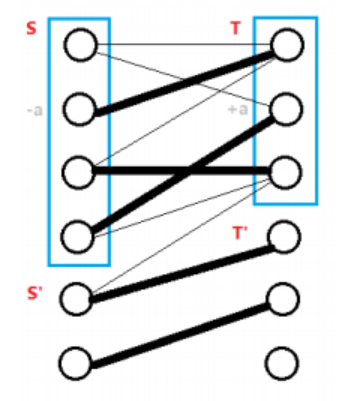
\includegraphics[width=0.3\textwidth,center]{../photo/km}\\
\indent此时无法继续修改,这时我们只能修改一些顶标使得相等子图发生变化从而可以继续匹配下去,这就意味着$S$中的某点必须做出让步,去匹配一些权值稍微低一点的边。我们找出$S\sim T'$中权值最小的边,权值$a=\min\{lx(u)+ly(v)-w(u,v)| u\in S,v\in T'\}$,使得损失尽可能降低。\\
\indent使$S$中的顶标$-a$,$T$中的顶标$+a$,可以发现:$S\sim T$边依然在相等子图中。$S' \sim T'$没有变化。$S\sim T'$的$lx+ly$减少,有可能加入相等子图。$S'\sim T$的边不可能加入相等子图。\\
\indent相等子图发生了变化,观察是否可以匹配,否则重复上述过程。由于原图一定存在完美匹配,所以最多$n$次一定可以找到增广路。\\
\indent一开始枚举$n$个点找增广路,为了找增广路需要延伸$n$次交错树,每次延伸需要$n$次维护,共$O(n^3)$。
\begin{lstlisting}[language=c++,escapeinside=``]
bool check(int v)
{
    visy[v]=1;
    if(maty[v]!=-1)
    {
        q.push(maty[v]);visx[maty[v]]=1;
        return false;
    }
    while(v!=-1){maty[v]=pre[v];swap(v,matx[pre[v]]);}
    return true;
}
void bfs(int x)
{
    while(!q.empty()) q.pop();
    q.push(x);visx[x]=1;
    while(1)
    {
        while(!q.empty())//`使用BFS进行匹配`
        {
            int u=q.front();q.pop();
            for(int v=1;v<=n;v++)
            {
                if(visy[v]) continue;
                int delta=lx[u]+ly[v]-side[u][v];
                if(slack[v]<delta) continue;
                pre[v]=u; //`delta=0意为改边属于相等子图`
                if(delta) slack[v]=delta;
                else if(check(v)) return;
            }
        }
        int mn=1e9;//匹配失败
        for(int i=1;i<=n;i++) if(!visy[i]) mn=min(mn,slack[i]);
        for(int i=1;i<=n;i++)
        {
            if(visx[i]) lx[i]-=mn;
            if(visy[i]) ly[i]+=mn;
            else slack[i]-=mn;
        }
        for(int i=1;i<=n;i++)
        {
            if (!visy[i]&&slack[i]==0&&check(i)) return;
        }
    }
}
void km()
{
    memset(lx,0,sizeof(lx));
    memset(ly,0,sizeof(ly));
    memset(matx,-1,sizeof(matx));
    memset(maty,-1,sizeof(maty));
    for(int i=1;i<=n;i++)
    {
        for(int j=1;j<=n;j++) lx[i]=max(lx[i],side[i][j]);
    }
    for(int i=1;i<=n;i++)
    {
        memset(visx,0,sizeof(visx));
        memset(visy,0,sizeof(visy));
        memset(slack,0x3f,sizeof(slack));
        bfs(i);//`slack[i]的值为右边第i个点和左边的点的顶标的最大值`
    }
    int ans=0;
    for(int i=1;i<=n;i++) ans+=side[i][matx[i]];
    printf("%d\n",ans);
    for(int i=1;i<=n;i++) printf("%d ",maty[i]);
}
\end{lstlisting}
\subsubsection{转化为费用流模型}
\indent在图中新增一个源点和一个汇点。\\
\indent从源点向二分图的每个左部点连一条流量为$1$,费用为$0$的边,从二分图的每个右部点向汇点连一条流量为$1$,费用为$0$的边。\\
\indent接下来对于二分图中每一条连接左部点$u$和右部$v$,边权为$w$的边,则连一条从$u$到$v$,流量为$1$,费用为$w$的边。\\
\indent求这个网络的\textbf{最大费用最大流}即可得到答案。
\subsection{一般图最大匹配}
\subsubsection{带花树}
\indent一般图匹配和二分图匹配不同的是,图可能存在奇环。时间复杂度$O(n^3)$\\
\begin{lstlisting}[language=c++,escapeinside=``]
int find(int x){return fa[x]==x?x:fa[x]=find(fa[x]);}
int LCA(int u,int v)
{
    ++tim;u=find(u);v=find(v);
    while(dfn[u]!=tim)//`u,v轮流上跳,直到跳到环顶`
    {
        dfn[u]=tim;
        u=find(pre[mat[u]]);
        if(v) swap(u,v);
    }
    return u;
}
void Blossom(int x,int y,int w)
{//对奇环进行缩花,同时将图上所有白点涂黑,向环外增广
    while(find(x)!=w)
    {
        pre[x]=y,y=mat[x];
        if(vis[y]==2) vis[y]=1,q.push(y);
        if(find(x)==x) fa[x]=w;
        if(find(y)==y) fa[y]=w;
        x=pre[y];
    }
}
int bfs(int x)
{
    for(int i=1;i<=n;i++) fa[i]=i,vis[i]=pre[i]=0;
    while(!q.empty()) q.pop(); q.push(x);vis[x]=1;
    while(!q.empty())
    {
        int u=q.front();q.pop();
        for(int i=head[u];~i;i=r[i].nex)
        {
            int v=r[i].b;
            //`u,v在同一朵花中或v是白色(偶环)`
            if(find(u)==find(v) || vis[v]==2) continue;
            if(!vis[v]) //`如果v尚未染色`
            {
                vis[v]=2;pre[v]=u;
                if(!mat[v])//增广成功
                {
                    for(int j=v,last;j;j=last) 
                    last=mat[pre[j]],mat[j]=pre[j],mat[pre[j]]=j;
                    return 1;
                }
                vis[mat[v]]=1;q.push(mat[v]);
            }
            else //`如果v是黑色,出现奇环,开花`
            {
                int w=LCA(v,u);//第一次进入奇环的黑点
                Blossom(u,v,w);Blossom(v,u,w);
            }
        }
    }
    return 0;
}
void match()
{
    int ans=0;
    for(int i=1;i<=n;i++) if(!mat[i] && bfs(i)) ans++;
    printf("%d\n",ans);
    for(int i=1;i<=n;i++) printf("%d ",mat[i]);
    puts("");
}
\end{lstlisting}
\section{网络流}
\subsection{最大流}
\subsubsection{EK算法}
EK算法就是BFS找增广路,然后对其进行增广,时间复杂度$O(nm^2)$。
\begin{lstlisting}[language=c++]
int bfs(int s,int t)
{
    memset(vis,0,sizeof(vis));
    queue<int>q;q.push(s);
    vis[s]=1;incf[s]=1e18;
    while(!q.empty())
    {
        int u=q.front();q.pop();
        for(int i=head[u];~i;i=r[i].nex)
        {
            int v=r[i].b;
            if(vis[v] || r[i].c==0) continue;
            q.push(v);vis[v]=1;pre[v]=i^1;
            incf[v]=min(incf[u],r[i].c);
            if(v==t) return 1;
        }
    }
    return 0;
}
int EK(int s,int t)
{
    int p=t;
    while(p!=s)
    {
        r[pre[p]].c+=incf[t];
        r[pre[p]^1].c-=incf[t];
        p=r[pre[p]].b;
    }
    return incf[t];
}
\end{lstlisting}
\subsubsection{Dinic算法}
\indent Dinic算法的过程是这样的:每次增广前,我们先用BFS来将图分层。设源点的层数为$0$,那么一个点的层数便是它离源点的最近距离。\\
\indent 然后使用DFS对流量进行增广,每次找增广路的时候,都只找比当前点层数多$1$的点进行增广(这样就可以确保我们找到的增广路是最短的),时间复杂度$O(n^2m)$。\\
\indent多路增广优化:每次找到一条增广路的时候,如果残余流量没有用完怎么办呢?我们可以利用残余部分流量,再找出一条增广路。这样就可以在一次DFS中找出多条增广路,大大提高了算法的效率。\\
\indent当前弧优化:如果一条边已经被增广过,那么它就没有可能被增广第二次。那么,我们下一次进行增广的时候,就可以不必再走那些已经被增广过的边。
\begin{lstlisting}[language=c++]
int make_level()
{
    memset(depth,-1,sizeof(depth));
    queue<int>q;q.push(s);
    depth[s]=1;now[s]=head[s];//当前弧优化
    while(!q.empty())
    {	
        int u=q.front();q.pop();
        for(int i=head[u];~i;i=r[i].nex)
        {
            int v=r[i].b;
            if(depth[v]!=-1 || r[i].c<=0) continue;
            now[v]=head[v];
            depth[v]=depth[u]+1;
            q.push(v);
        }
    }
    return depth[t]!=-1;
}
int dinic(int u,int flow)
{
    if(u==t) return flow;
    int sum=0;
    for(int i=now[u];~i;i=r[i].nex)//多路增广
    {
        now[u]=i;
        int v=r[i].b;
        if(depth[v]!=depth[u]+1 || r[i].c<=0) continue;
        int use=dinic(v,min(flow-sum,r[i].c));
        if(use)
        {
            r[i].c-=use;r[i^1].c+=use;
            sum+=use;
        }
        if(sum==flow) return flow;
    }
    if(sum==0) depth[u]=-1;
    return sum;
}
\end{lstlisting}
\subsubsection{ISAP}
\indent在Dinic算法中,我们每次求完增广路后都要跑BFS来分层,有没有更高效的方法呢?ISAP是一种只需要一次BFS就可以不断增广的写法。\\
\indent和Dinic算法一样,我们还是先跑BFS对图上的点进行分层,不过与Dinic略有不同的是,我们选择在反图上,从$t$点向$s$点进行BFS。\\
\indent设$i$号点的层为$d_i$,当我们结束在$i$号点的增广过程后,我们遍历残量网络上$i$的所有出边,找到层最小的出点$j$,随后令$d_i=d_j+1$。特别地,若残量网络上$i$无出边,则$d_i=n$。时间复杂度$O(n^3)$\\
\indent GAP优化:记录每一层的点的数量,若某层为空,即出现了断层,直接结束。
\begin{lstlisting}[language=c++,escapeinside=``]
void make_level()
{
    queue<int>q;q.push(t);
    depth[t]=1;gap[1]++;
    while(!q.empty())
    {
        int u=q.front();q.pop();
        for(int i=head[u];~i;i=r[i].nex)
        {
            int v=r[i].b;
            if(depth[v]) continue;
            depth[v]=depth[u]+1;
            gap[depth[v]]++;
            q.push(v);
        }
    }
}
ll dfs(ll u,ll flow)
{
    if(u==t) return flow;
    ll sum=0;
    for(int i=head[u];~i;i=r[i].nex)
    {
        ll v=r[i].b;
        if(depth[v]+1!=depth[u] || r[i].c==0) continue;
        ll use=dfs(v,min(flow-sum,r[i].c));
        if(use)
        {
            r[i].c-=use;
            r[i^1].c+=use;
            sum+=use;
        }	
        if(sum==flow) return flow;
    }
    gap[depth[u]]--;
    if(gap[depth[u]==0]) depth[s]=n+1;//GAP优化
    depth[u]++;gap[depth[u]]++;
    return sum;
}
void ISAP()
{
    make_level();
    while(depth[s]<=n) 
    {
        ans+=dfs(s,1e18);
    }
}
\end{lstlisting}
\subsubsection{HPLL}
时间复杂度$O(n^2\sqrt m)$
\begin{lstlisting}[language=c++]
#include<bits/stdc++.h>
using namespace std;
const int N = 1200, M = 120000, INF = 0x3f3f3f3f;
int n, m, s, t;
struct qxx {int nex, t, v;};
qxx e[M * 2 + 1];
int h[N + 1], cnt = 1;
void add_path(int f, int t, int v) { 
    e[++cnt] = (qxx){h[f], t, v}, h[f] = cnt; }
void add_flow(int f, int t, int v) {
    add_path(f, t, v);
    add_path(t, f, 0);
}
int ht[N + 1], ex[N + 1],
    gap[N];  // 高度; 超额流; gap 优化 gap[i] 为高度为 i 的节点的数量
stack<int> B[N];  // 桶 B[i] 中记录所有 ht[v]==i 的v
int level = 0;    // 溢出节点的最高高度
int push(int u) {      // 尽可能通过能够推送的边推送超额流
    bool init = u == s;  // 是否在初始化
    for (int i = h[u]; i; i = e[i].nex) {
        const int &v = e[i].t, &w = e[i].v;
        if (!w || init == false && ht[u] != ht[v] + 1)  // 初始化时不考虑高度差为1
        continue;
        int k = init ? w : min(w, ex[u]);
        // 取到剩余容量和超额流的最小值,初始化时可以使源的溢出量为负数。
        if(v!=s && v!=t && !ex[v]) B[ht[v]].push(v),level= max(level, ht[v]);
        ex[u] -= k, ex[v] += k, e[i].v -= k, e[i ^ 1].v += k;  // push
        if (!ex[u]) return 0;  // 如果已经推送完就返回
    }
    return 1;
}
void relabel(int u) {  // 重贴标签(高度)
    ht[u] = INF;
    for (int i = h[u]; i; i = e[i].nex)
        if (e[i].v) ht[u] = min(ht[u], ht[e[i].t]);
    if (++ht[u] < n) {  // 只处理高度小于 n 的节点
        B[ht[u]].push(u);
        level = max(level, ht[u]);
        ++gap[ht[u]];  // 新的高度,更新 gap
    }
}
bool bfs_init() {
    memset(ht, 0x3f, sizeof(ht));
    queue<int> q;
    q.push(t), ht[t] = 0;
    while (q.size()) {  // 反向 BFS, 遇到没有访问过的结点就入队
        int u = q.front();
        q.pop();
        for (int i = h[u]; i; i = e[i].nex) {
        const int &v = e[i].t;
        if (e[i ^ 1].v && ht[v] > ht[u] + 1) ht[v] = ht[u] + 1, q.push(v);
        }
    }
    return ht[s] != INF;  // 如果图不连通,返回 0
}
// 选出当前高度最大的节点之一, 如果已经没有溢出节点返回 0
    int select() {
    while (B[level].size() == 0 && level > -1) level--;
    return level == -1 ? 0 : B[level].top();
}
int hlpp() {                  // 返回最大流
    if (!bfs_init()) return 0;  // 图不连通
    memset(gap, 0, sizeof(gap));
    for (int i = 1; i <= n; i++)
        if (ht[i] != INF) gap[ht[i]]++;  // 初始化 gap
    ht[s] = n;
    push(s);  // 初始化预流
    int u;
    while ((u = select())) {
        B[level].pop();
        if (push(u)) {  // 仍然溢出
        if (!--gap[ht[u]])
            for (int i = 1; i <= n; i++)
            if (i != s && i != t && ht[i] > ht[u] && ht[i] < n + 1)
                ht[i] = n + 1;  // 这里重贴成 n+1 的节点都不是溢出节点
        relabel(u);
        }
    }
    return ex[t];
}
int main() {
    scanf("%d%d%d%d", &n, &m, &s, &t);
    for (int i = 1, u, v, w; i <= m; i++) {
        scanf("%d%d%d", &u, &v, &w);
        add_flow(u, v, w);
    }
    printf("%d", hlpp());
    return 0;
}
\end{lstlisting}
\subsection{最小割}
对于一个网络流图$G=(V,E)$,其割的定义为一种点的划分方式:将所有的点划分为$S$和$T=V-S$两个集合,其中源点$s\in S$,汇点$t \in T$。
\subsubsection{方案}
我们可以通过从源点$s$开始DFS,每次走残量大于$0$的边,找到所有$S$点集内的点。
\begin{lstlisting}[language=c++]
void dfs(int u)
{
    vis[u]=1;
    for(int i=head[u];~i;i=r[i].nex)
    {
        int v=r[i].b;
        if(!vis[v]&&r[i].c) dfs(v);
    }
}
\end{lstlisting}
\subsubsection{割边数量}
如果需要在最小割的前提下最小化割边数量,那么先求出最小割,把没有满流的边容量改成$inf$,满流的边容量改成$1$,重新跑一遍最小割就可求出最小割边数量;如果没有最小割的前提,直接把所有边的容量设成$1$,求一遍最小割就好了。
\subsubsection{问题模型1:二者选其一}
\indent有$n$个物品和两个集合$A,B$,如果一个物品没有放入$A$集合会花费$a_i$,没有放入$B$集合会花费$b_i$;还有若干个形如$u_i,v_i,w_i$限制条件,表示如果$u_i$和$v_i$同时不在一个集合会花费$w_i$。每个物品必须且只能属于一个集合,求最小的代价。\\
\indent我们对于每个集合设置源点$s$和汇点$t$,第$i$个点由$s$连一条容量为$a_i$的边、向$t$连一条容量为$b_i$的边。对于限制条件$u,v,w$,我们在$u,v$之间连容量为$w$的双向边。\\
\indent最小割就是最小花费。
\subsubsection{问题模型2:最大权闭合图}
\indent最大权值闭合图,即给定一张有向图,每个点都有一个权值(可以为正或负或$0$),你需要选择一个权值和最大的子图,使得子图中每个点的后继都在子图中。\\
\indent做法:建立超级源点$s$和超级汇点$t$,若节点$u$权值为正,则$s$向$u$连一条有向边,边权即为该点点权;若节点$u$权值为负,则由$u$向$t$连一条有向边,边权即为该点点权的相反数。原图上所有边权改为$inf$。跑网络最大流,将所有正权值之和减去最大流,即为答案。\\
\indent此外,该图应该是一个拓扑图,如果无法满足则应该先拓扑排序找出合法的边。\\
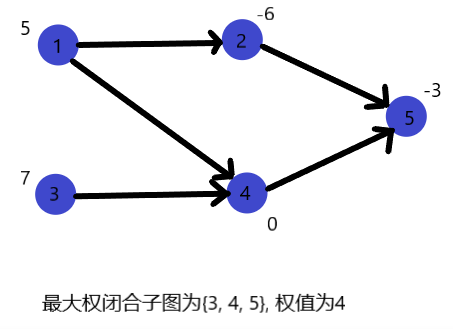
\includegraphics[width=0.4\textwidth,center]{../photo/zxg1}
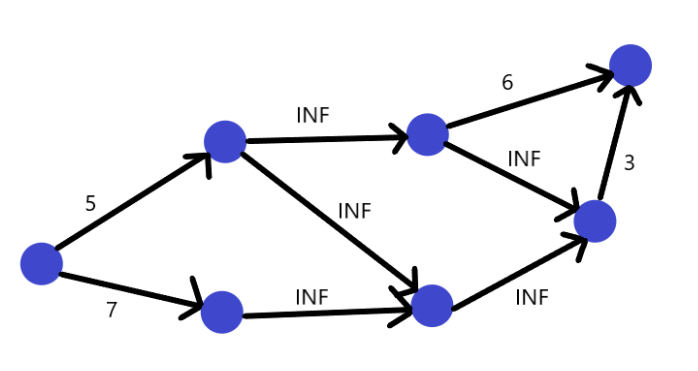
\includegraphics[width=0.5\textwidth,center]{../photo/zxg2}\\
\indent判断一条边是否被割,应该通过最后一次增广后,depth是否为$-1$来判断。
\subsection{费用流}
只需将EK算法或Dinic算法中找增广路的过程,替换为用最短路/最长路算法寻找单位费用最小的增广路即可。
\begin{lstlisting}[language=c++,title=最小费用最大流]
bool spfa()
{
    for(int i=1;i<=n;i++)
    {
        pre[i]=-1;vis[i]=0;dis[i]=inf;
    }
    incf[s]=inf;
    queue<int>q;q.push(s);
    dis[s]=0;vis[s]=1;
    while(!q.empty())
    {
        int u=q.front();q.pop();
        vis[u]=0;
        for(int i=head[u];~i;i=r[i].nex)
        {
            int v=r[i].b;
            if(r[i].c && dis[v]>dis[u]+r[i].d)
            {
                dis[v]=dis[u]+r[i].d;
                incf[v]=min(incf[u],r[i].c);
                pre[v]=i;
                if(vis[v]==0)
                {
                    vis[v]=1;
                    q.push(v);
                }
            }
        }
    }
    if(pre[t]==-1) return false;
    return true;
}
void MCMF()
{
    while(spfa())
    {
        int x=t;
        maxflow+=incf[t];
        mincost+=incf[t]*dis[t];
        while(x!=s)
        {
            r[pre[x]].c-=incf[t];
            r[1^pre[x]].c+=incf[t];
            x=r[1^pre[x]].b;
        }
    }
}
\end{lstlisting}
\subsection{上下界网络流}
\subsubsection{无源汇上下界可行流}
\indent给定无源汇流量网络$G$。询问是否存在一种标定每条边流量的方式,使得每条边流量满足上下界同时每一个点流量平衡(循环环流)。一个满足流量平衡的点意味着该点的流入流量等于流出流量。\\
\indent首先每条边的流量应该大于其下界流量。假设每条边当前都只流出了其下界,用下界流量记录各点的流量平衡状态。在这个条件的基础上建立一个新图,新图每条边的流量为:流量上界$-$流量下界,也就是图上剩余的流量值。\\
\indent建立虚拟源汇点$S',T'$。若点$u$流出量大于流入量,差值为$M$,我们就从$S'$出发向$u$连接一条值为$M$的附加边。若点$u$流出量小于流入量,差值为$M$,我们就从$u$出发向$T'$连接一条值为$M$的附加边。\\
\indent如果附加边满流,说明这一个点的流量平衡条件可以满足,否则这个点的流量平衡条件不满足。在建图完毕之后跑$S'$到$T'$的最大流,若$S'$连出去的边全部满流,则存在可行流,否则不存在。
\subsubsection{有源汇上下界可行流}
\indent给定有源汇流量网络$G$。询问是否存在一种标定每条边流量的方式,使得每条边流量满足上下界同时除了源点和汇点每一个点流量平衡。\\
\indent假设源点为$S$,汇点为$T$。则我们可以加入一条$T$到$S$的上界为$\infty$,下界为$0$的边转化为无源汇上下界可行流问题。若有解,则$S$到$T$的可行流流量等于$T$到$S$的附加边的流量。
\subsubsection{有源汇上下界最大流}
\indent首先,先判断是否存在有源汇上下界可行流。如果找不到解就可以直接结束。\\
\indent记计算出来的上下界可行流为$flow1$。否则,我们删去图上所有的附加边,在残量网络上算出$S$到$T$计算出最大流$flow2$。有源汇上下界最大流$=flow1+flow2$。
\begin{lstlisting}[language=C++,title=有源汇上下界最大流]
#include<bits/stdc++.h>
#define inf 0x3f3f3f3f
using namespace std;
int n,m,in[205],out[205],depth[205],now[205],head[205],s,t,num,low[200005];
struct road{int b,c,nex;}r[200005];
void add(int a,int b,int c){
    r[num].b=b;r[num].c=c;r[num].nex=head[a];head[a]=num++;}
int make_level()
{
    memset(depth,-1,sizeof(depth));
    queue<int>q;q.push(s);
    depth[s]=1;now[s]=head[s];
    while(!q.empty())
    {	
        int u=q.front();q.pop();
        for(int i=head[u];~i;i=r[i].nex)
        {
            int v=r[i].b;
            if(depth[v]!=-1 || r[i].c<=0) continue;
            now[v]=head[v];
            depth[v]=depth[u]+1;
            q.push(v);
        }
    }
    return depth[t]!=-1;
}
int dinic(int u,int flow)
{
    if(u==t) return flow;
    int sum=0;
    for(int i=now[u];~i;i=r[i].nex)
    {
        now[u]=i;
        int v=r[i].b;
        if(depth[v]!=depth[u]+1 || r[i].c<=0) continue;
        int use=dinic(v,min(flow-sum,r[i].c));
        if(use)
        {
            r[i].c-=use;r[i^1].c+=use;
            sum+=use;
        }
        if(sum==flow) return flow;
    }
    if(sum==0) depth[u]=-1;
    return sum;
}
int main()
{
    memset(head,-1,sizeof(head));
    scanf("%d%d%d%d",&n,&m,&s,&t);
    for(int i=1;i<=m;i++)
    {
        int a,b,u;scanf("%d%d%d%d",&a,&b,&low[i],&u);
        add(a,b,u-low[i]);add(b,a,0);
        out[a]+=low[i];in[b]+=low[i];//记录各点的流量进出状况
    }
    int s1=n+1,t1=s1+1;
    int sum=0,st=num;
    for(int i=1;i<=n;i++)
    {
        if(in[i]==out[i]) continue;//建立附加边
        if(in[i]>out[i]) add(s1,i,in[i]-out[i]),add(i,s1,0);
        else add(i,t1,out[i]-in[i]),add(t1,i,0),sum+=abs(in[i]-out[i]);
    }
    add(t,s,inf);add(s,t,0);//建立附加边
    int ans=0;
    swap(s,s1);swap(t,t1);
    while(make_level()) ans+=dinic(s,1e9);
    if(ans==sum)//存在可行流
    {
        int flow1=r[num-1].c;
        for(int i=st;i<num;i++) r[i].c=0; //删除图上所有的附加边
        swap(s,s1);swap(t,t1);
        while(make_level()) flow1+=dinic(s,inf); //flow1+flow2
        printf("%d\n",flow1);
    }
    else//不存在可行流
        puts("please go home to sleep");
}
\end{lstlisting}
\subsubsection{有源汇上下界最小流}
\indent首先,先判断是否存在有源汇上下界可行流。如果找不到解就可以直接结束。\\
\indent记计算出来的上下界可行流为$flow1$。否则,我们删去图上所有的附加边,在残量网络上算出$T$到$S$计算出最大流$flow2$。意为将多余的无用流量退还回去,有源汇上下界最大流$=flow1-flow2$。
\section{Stoer-Wagner算法}
\indent Stoer-Wagner算法是一种解决无向正权图上的\textbf{全局最小割}问题的算法。算法复杂度$O(nm+n^2\log|n|)$一般可近似看作$O(n^3)$。\\
\noindent\textbf{算法过程:}\\
\indent1.在图$G$中任意指定两点$s,t$,并且以这两点作为源汇点求出最小割,更新当前答案。\\
\indent2.将$t$合并入$s$变为同一点。合并过程:删除$s,t$之间的连边,对于$G/{s,t}$中任意一点$k$,删除$t,k$,并将其边权$d(t,k)$加到$d(s,k)$上。\\
\indent3.输出所有最小割的最小值。\\
\indent若选择的割边会将两点$s,t$分为两个连通块,则该割边的大小即以$s,t$为源汇的最小割。否则,$s,t$将绑定在一起,共享所有的边。因此,处理完一对$s,t$之间的最小割后,就只有它们处于同一连通块的情况了,也就是做完一对以后就合并一对点,如是进行次$n-1$即合并成一个点,算法完成。\\
\noindent\textbf{最小割求法:}\\
\indent假设进行若干次合并以后,当前图$G'=(V',E')$,我们构造一个集合$A$,初始时令$A=\varnothing$。\\
\indent我们每次将$G'$中所有点中,满足$i\notin A$,且权值函数$w(i)$最大的节点加入集合$A$,直到$|A|=|V'|$。\\
\indent其中$w(i)=\displaystyle\sum_{j\in A}d(i,j)$。\\
\indent令$ord(i)$表示第$i$个加入$A$的点,令$s$为$ord(|V'-1|)$,$t$为$ord(|V'|)$,则此时的$w(t)$就是$s$到$t$的最小割。
\begin{lstlisting}[language=c++,escapeinside=``]
int contract(int x) 
{
    memset(vis,0,sizeof(vis));
    memset(w,0,sizeof(w));
    w[0]=-1;
    for(int i=1;i<=n-x+1;i++) 
    {
        int mx=0;
        for (int j=1;j<=n;j++) 
        {   //`dap[j]=1表示j点已经与其他点合并`
            if(!dap[j]&&!vis[j]&&w[j]>w[mx]) mx=j;
        }
        vis[mx]=1,ord[i]=mx; //`第i个加入集合A的点是ord[i]`
        for(int j=1;j<=n;j++) 
        {
            if(!dap[j]&&!vis[j]) w[j]+=side[mx][j]; //`更新维护w函数`
        }
    }
    s=ord[n-x],t=ord[n-x+1]; //`这样的s和t的最小割一定是w[t]`
    return w[t];
}
int Stoer_Wagner() 
{
    int res=INF;
    for (int i=1;i<n;i++) 
    {
        res=min(res,contract(i));
        dap[t]=1; //`将t与s合并`
        for (int j=1;j<=n;j++) 
        {
            side[s][j]+=side[t][j];
            side[j][s]+=side[j][t];
        }
    }
    return res;
}
\end{lstlisting}
\section{特殊的图}
\subsection{竞赛图}
竞赛图也叫有向完全图。每对顶点之间都有一条边相连的有向图称为竞赛图。
\begin{itemize}
    \item 竞赛图没有自环,没有二元环;若竞赛图存在环,则一定存在三元环。(如果存在一个环大于三元,那么一定存在另一个三元的小环。)
    \item 任意竞赛图都有哈密顿路径(经过每个点一次的路径,不要求回到出发点)。
    \item 图存在哈密顿回路的充要条件是强联通。
\end{itemize}
\subsubsection{兰道定理}
兰道定理是用来判定竞赛图的定理。将一个竞赛图的每一个点的出度从小到大排序后得到长度为$n$的序列称为竞赛图的比分序列$s={s_1\leq s_2 \leq \cdots \leq s_n}$是合法的比分序列当且仅当:
$$
\forall 1\leq k \leq n,\sum_{i=1}^{k} s_i \ge\binom{k}{2} 
$$
且$k=n$时一定相等。
\subsection{平面图}
\indent如果可以将一个图画在二维平面上,可以存在一种画法使任意两条边都不相交,该图就是平面图。\\
\subsubsection{如何判断一个图是不是平面图?}
\noindent拓扑学欧拉公式:对于一个连通平面图$G=(V,E,F),|V|-|E|+|F|=2$则该图为平面图,其中$|V|,|E|,|F|$分别为点数,边数,和形成的面数(面内不应该有其余的边,且最外面的无限大的区域也算一个面)。\\
\noindent证明:对于一棵树,一定是平面图,且满足$|V|-|E|+|F|=2$,此后,每增加一条边,都会多一条边和一个面。平面图边数和点数的关系:$m \leq 3*n-6$。
\subsection{对偶图}
对偶图是与平面图相伴的一种图。将平面图中的每个面都变为一个点,将各个面割开的边变为新的边,权值不变,连接在新的点上。对偶图的对偶图是原图。\\
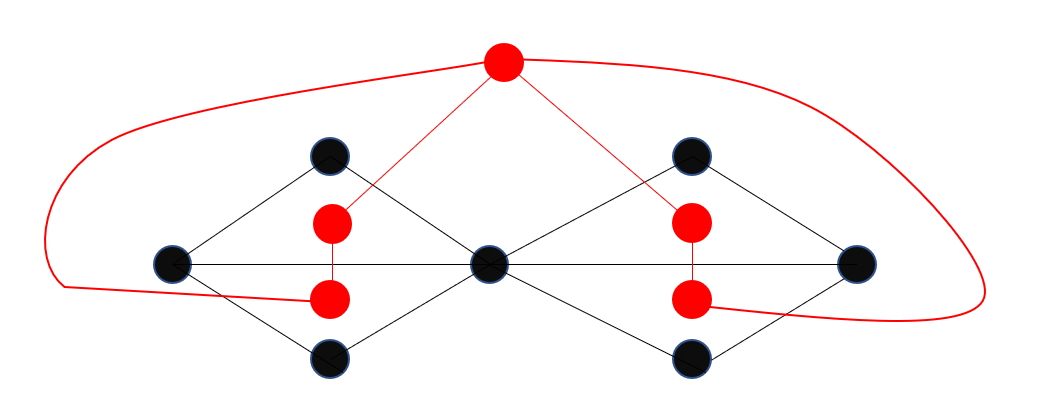
\includegraphics[width=0.5\textwidth,center]{../photo/duiou.png}
\subsubsection{平面图的最小割等于其对偶图的最短路}
对于一个$s-t$平面图,我们对其进行如下改造:首先连接$s-t$得到一个附加面,求该图的对偶图$G$,令附加面对应的点为$s$,无界面对应的点为$t$,然后对图$G$进行连边,此时$s-t$最短路就是最小割。\\
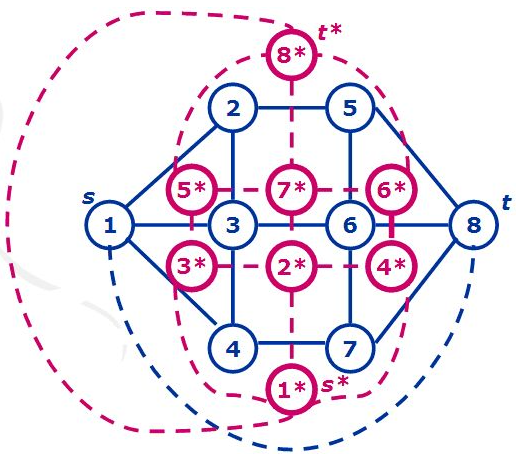
\includegraphics[width=0.5\textwidth,center]{../photo/duiou2.png}
\section{最小环}
给出一个图,问其中的有$n$个节点构成的边权和最小的环$(n\ge3)$是多大。二元化较为特殊,处理方法也比较简单。
\subsubsection{Dijkstra}
设$u$和$v$之间有一条边长为$w$的边,$dis(u,v)$表示删除$u$和$v$之间的连边之后,两点之间的最短路。那么图中的最小环是$dis(u,v)+w$。时间复杂度$O(m(n+m)\log n)$。
\subsubsection{floyd}
\begin{lstlisting}[language=c++,escapeinside=``]
int val[maxn+1][maxn+1]; //原图的邻接矩阵
int floyd(int &n) 
{
    int dis[maxn+1][maxn+1]; //最短路矩阵
    for(int i=1;i<=n;++i)
        for(int j=1;j<=n;++j) dis[i][j]=val[i][j]; //初始化最短路矩阵
    int ans=inf;
    for(int k=1;k<=n;++k) 
    {
        for(int i=1;i<k;++i)
            for(int j=1;j<i;++j)
            ans=min(ans,dis[i][j]+val[i][k]+val[k][j]); //更新答案
        for(int i=1;i<=n;++i)
            for(int j=1;j<=n;++j)
            dis[i][j]=min(dis[i][j],dis[i][k]+dis[k][j]);
    }
    return ans;
}
\end{lstlisting}
\ifx\allfiles\undefined
\end{document}
\fi


